\chapter{Experimental Results}
\markright{Experimental Results}
\label{exp}
\phantomsection
%\addcontentsline{toc}{chapter}{experiments}

The proposed method has been tested to verify the uniqueness of the watermark, i.e. if the detector presents a significantly higher score only in correspondence of the reference watermark. Moreover, we tested its validity in terms of robustness, in other words, the ability of the watermark to cope with the degradation of the frames due to malicious attacks such as spatial filtering, geometric transformation, compression and view synthesis. \newline 
In particular, in this thesis we tested the robustness against compression and view synthesis; in addition to the generated compressed videos, the YouTube video compression has been investigated. This choice has been made on the basis that nowadays YouTube is one of the most used video-sharing platform, representing a typical scenario of video distribution.\\
Another important feature of a good watermarking method is the perceptual transparency, such that human eye could not distinguish the dissimilarities between the watermarked image and the original one.\newline
In this chapter will be presented the results carried out to test both the spatial and frequency disparity-coherent watermarking algorithm performances.\newline

The experimental results have been proposed on a 1' stereo video sequence with a resolution of 1280x480. The video has been created with the \texttt{ffmpeg} library \cite{ffmpeg} and the input images are the stereo pairs in the New Tsukuba dataset \cite{tsu}; this dataset contains 1800 stereo pairs of resolution 640x480, with ground truth disparity maps, occlusion maps and discontinuity maps.\\
Ffmpeg is a library of the multimedia framework FFmpeg, able to decode, encode, transcode, mux, demux, stream, filter and play; ffmpeg is a command-line tool that converts audio or video formats and allows, among a various number of options, to choose the number of Group Of Picture's frame, the Constant Rate Factor value, the pixel format, the video coding format and the frame rate.\\
In video coding the Group Of Picture (GOP) is a group of successive pictures within a coded video stream. Each coded video stream consists of successive GOPs. From the pictures contained in it, the visible frames are generated.\\
GOP can contain the following picture types:
I frame (intra coded picture) is  a picture that is coded independently of all other pictures. Each GOP begins (in decoding order) with this type of picture; P frame (predictive coded picture) – contains motion-compensated difference information relative to previously decoded pictures;  B frame (bipredictive coded picture) contains motion-compensated difference information relative to previously decoded pictures. An I frame indicates the beginning of a GOP. Afterwards several P and B frames follow.\\
Constant Rate Factor (CRF) is the default quality setting for the x264 encoder; its value can be set in a range between 0 and 51, where lower values would result in better quality (at the expense of higher file sizes). Sane values are between 18 and 28. \\
Pixel format specifies the format of the color data for each pixel in the image, such as rgb24, yuv422p, yuva420p.\\
Video coding format is a content representation format for storage or transmission of digital video content; examples of video coding formats include MPEG-2 Part 2, MPEG-4 Part 2, H.264.\\
Frame rate is the frequency (rate) at which an imaging device displays frames.\\

In this work a Group Of Picture (GOP) of 60 frames, a frame rate of 30 fps, a pixel format yuv420p, the video codec H.264 and a CRF initial value of 1 have been chosen.\newline 
The video sequence has been marked every 60 frames, i.e. only the I frame of each GOP are marked.\newline 
With these settings a total number of 30 frame has been marked.\\
The watermark has been inserted with increasing values of the power and then the watermarked videos have been compressed with different levels of compression; higher values of the power lead in video visual degradation but make the watermark more robust against compression. \newline 
The compressed videos are obtain by changing the CRF value in the ffmpeg command line.



\section{Uniqueness of the watermark}

The first experiment we present aims to demonstrate the uniqueness of the watermark. We can say a mark is unique if the detector will present a significantly higher score only in correspondence of the reference watermark. 

Figures \ref{fig:Lr}-\ref{fig:Ll} show the response of the frequency watermark detector, in terms of loglikelihood value, to 100 randomly generated watermarks of which only one matches the reference watermark. Figure \ref{fig:Lnm} show the loglikelihood value when the image does not contain the watermark.

\begin{figure*}[h!]
    \centering
    \begin{subfigure}[t]{0.5\textwidth}
        \centering
       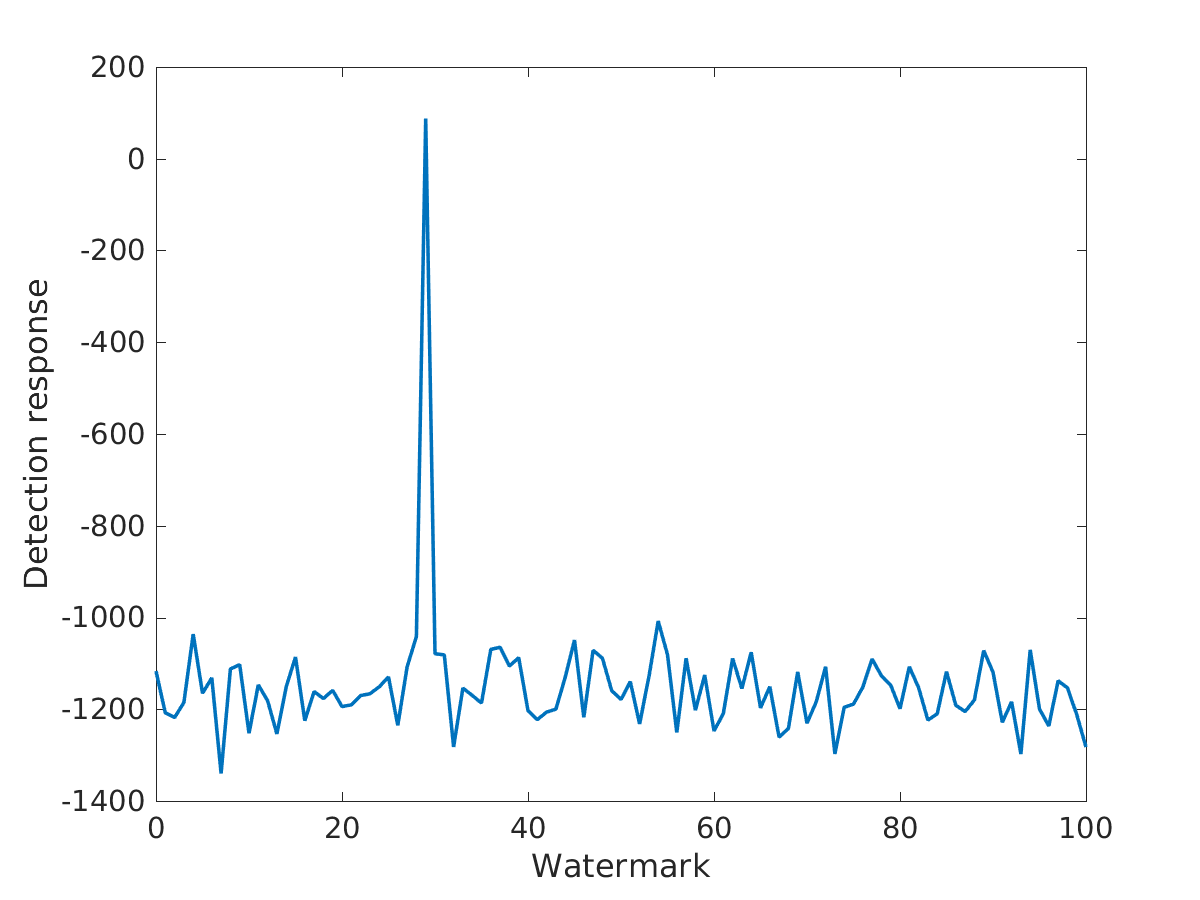
\includegraphics[width=1\textwidth]{./img/likelihood/correct_LikelihoodL_03.png}
          \caption{\small{detection on the left view}}
          \label{fig:Ll03}

    \end{subfigure}%
    ~ 
    \begin{subfigure}[t]{0.5\textwidth}
        \centering
        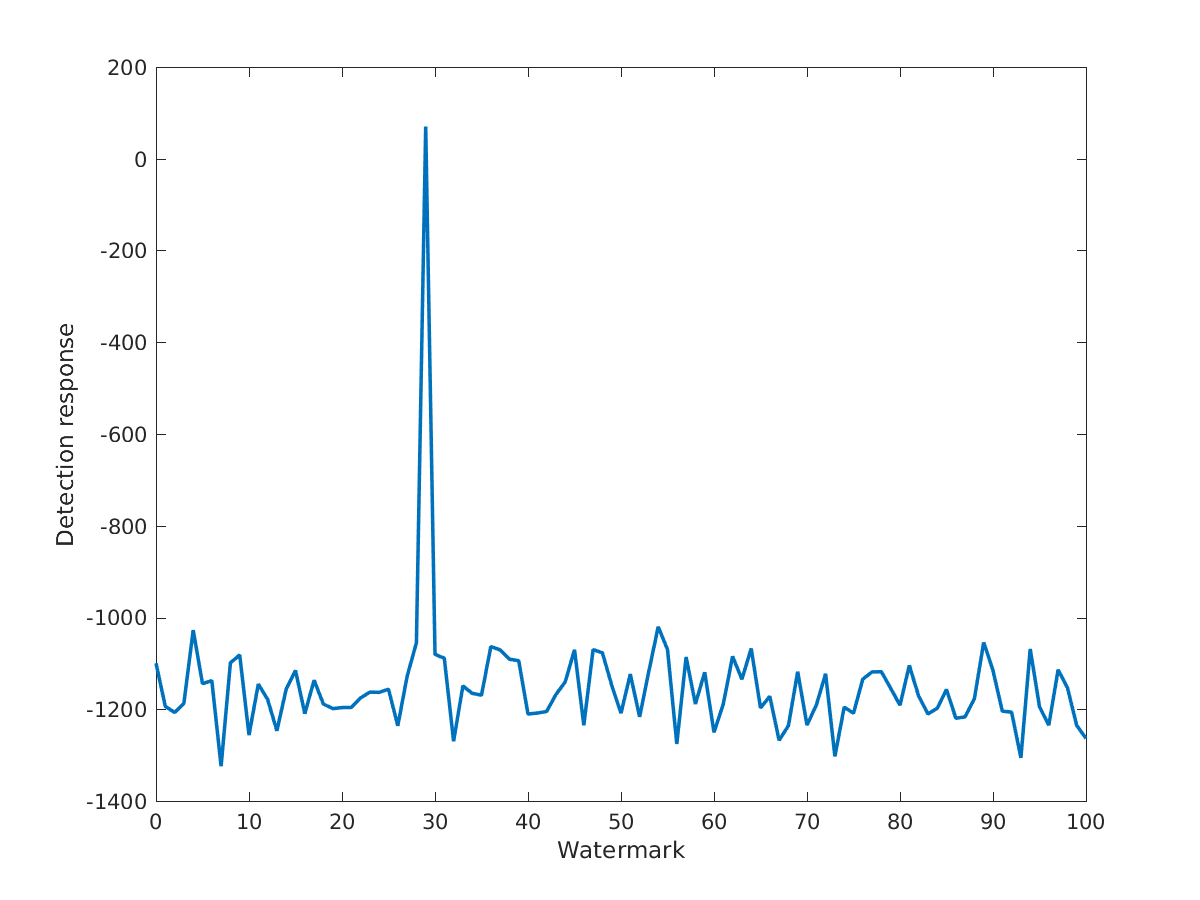
\includegraphics[width=1\textwidth]{./img/likelihood/correct_LikelihoodLr_03.png}
           \caption{\small{detection on the right view}}
           \label{fig:Lr03}
    \end{subfigure}
    \caption{Detector response on the left and right views marked with power equal to 0.3}
     \label{fig:Lr}
\end{figure*}
\begin{figure*}[h!]
    \centering
    \begin{subfigure}[t]{0.5\textwidth}
        \centering
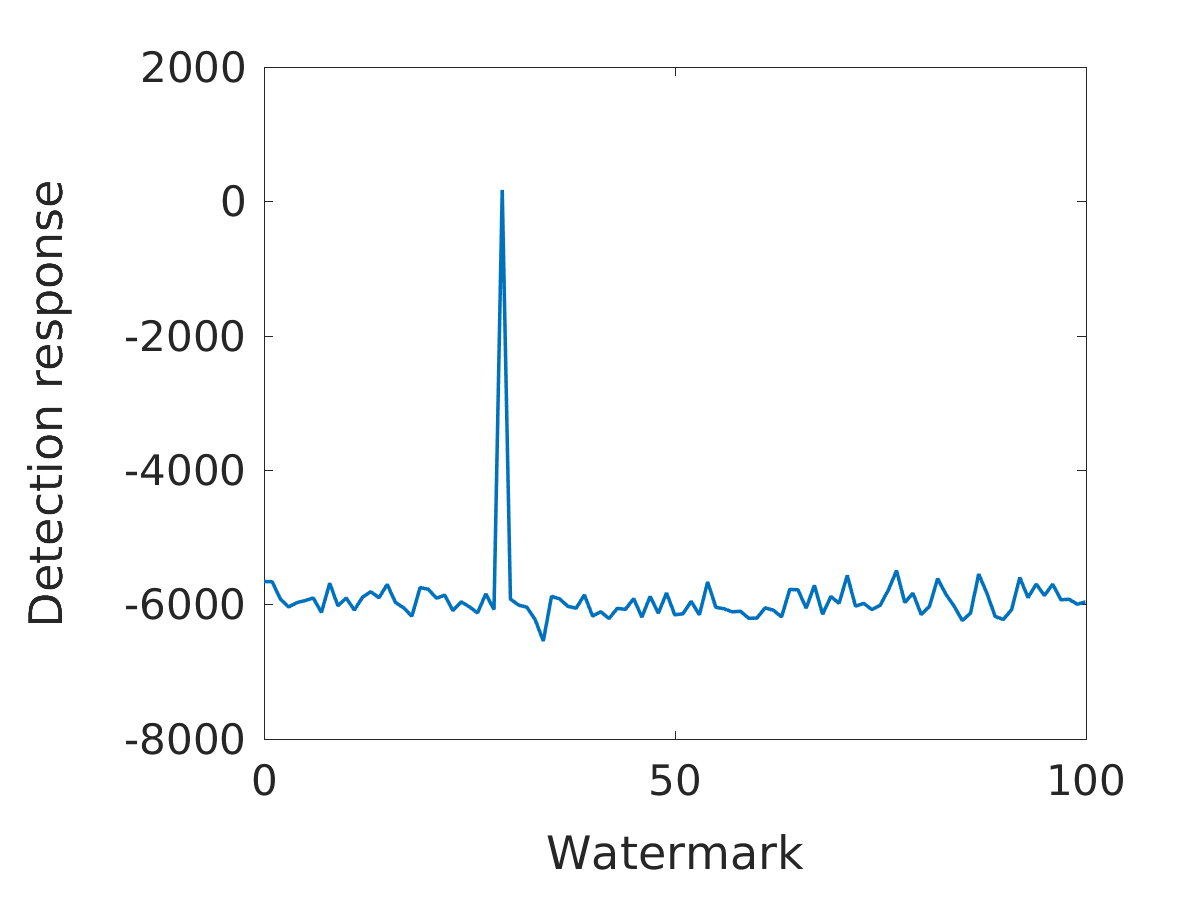
\includegraphics[width=1\textwidth]{./img/likelihood/correct_LikelihoodL_06.png}
          \caption{\small{detection on the left view}}
\label{fig:Ll06}

    \end{subfigure}%
    ~ 
    \begin{subfigure}[t]{0.5\textwidth}
        \centering
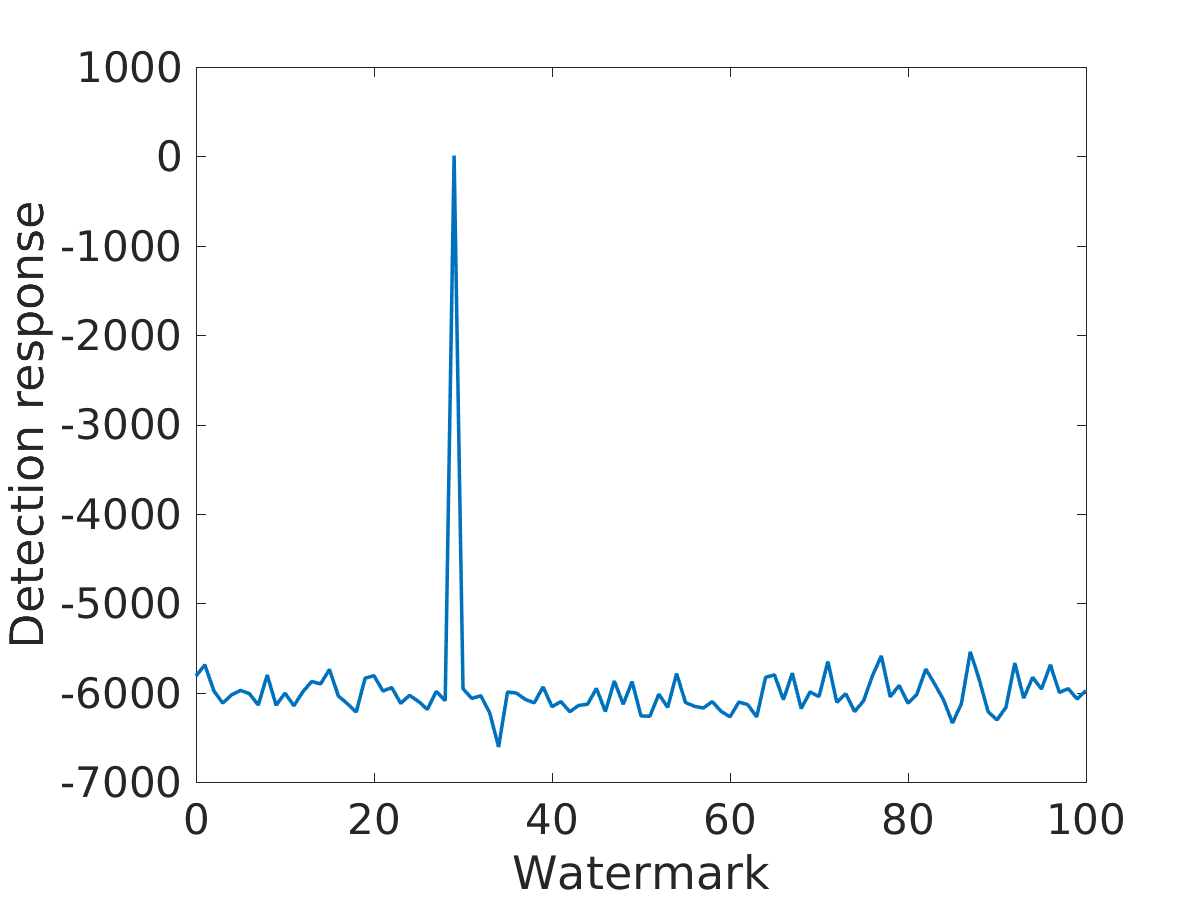
\includegraphics[width=1\textwidth]{./img/likelihood/correct_LikelihoodLr_06.png}
           \caption{\small{detection on the right view}}
\label{fig:Lr06}
    \end{subfigure}
    \caption{Detector response on the left and right views marked with power equal to 0.6}
     \label{fig:Ll}
\end{figure*}


\begin{figure*}[h!]
    \centering
    \begin{subfigure}[t]{0.5\textwidth}
        \centering
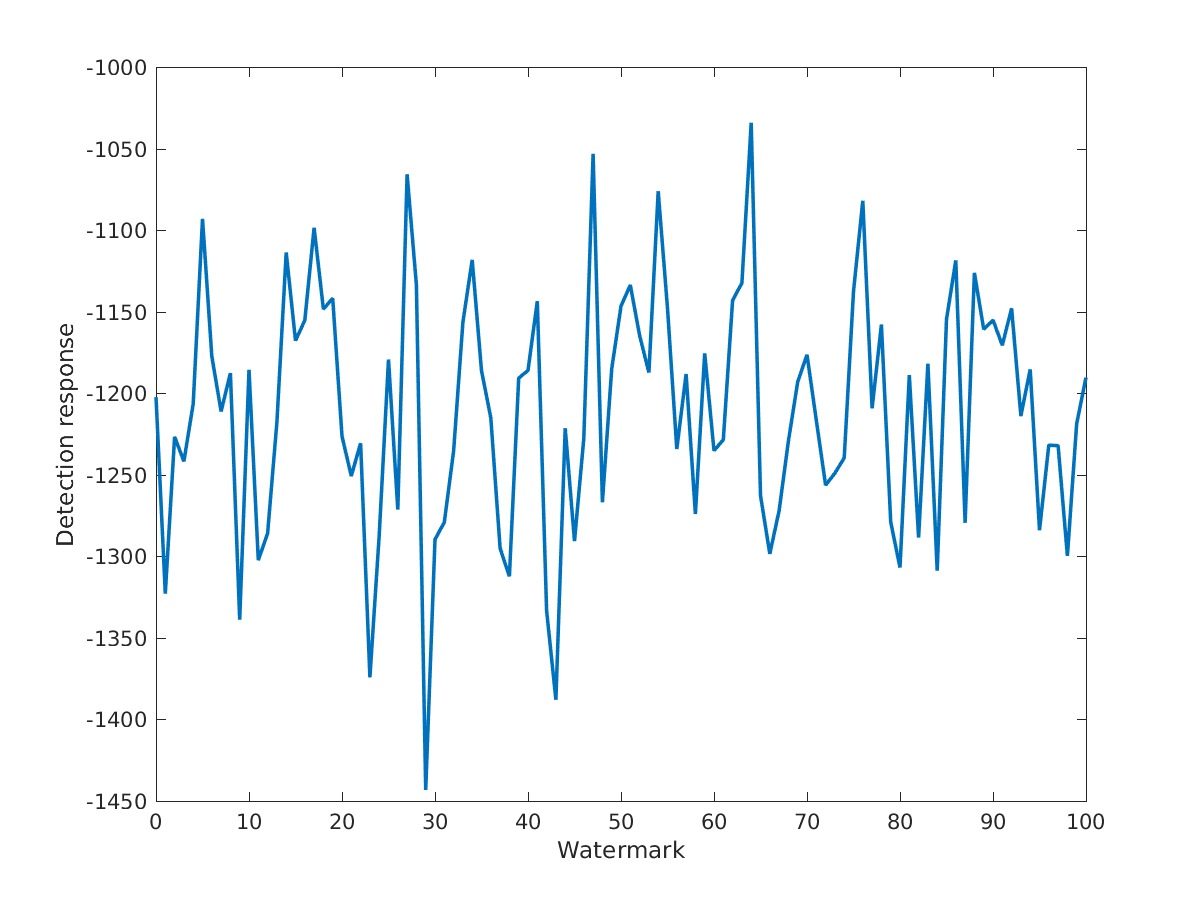
\includegraphics[width=1\textwidth]{./img/likelihood/correct_LikelihoodL_NM.png}
          \caption{\small{detection on the left view}}
\label{fig:Llnm}

    \end{subfigure}%
    ~ 
    \begin{subfigure}[t]{0.5\textwidth}
        \centering
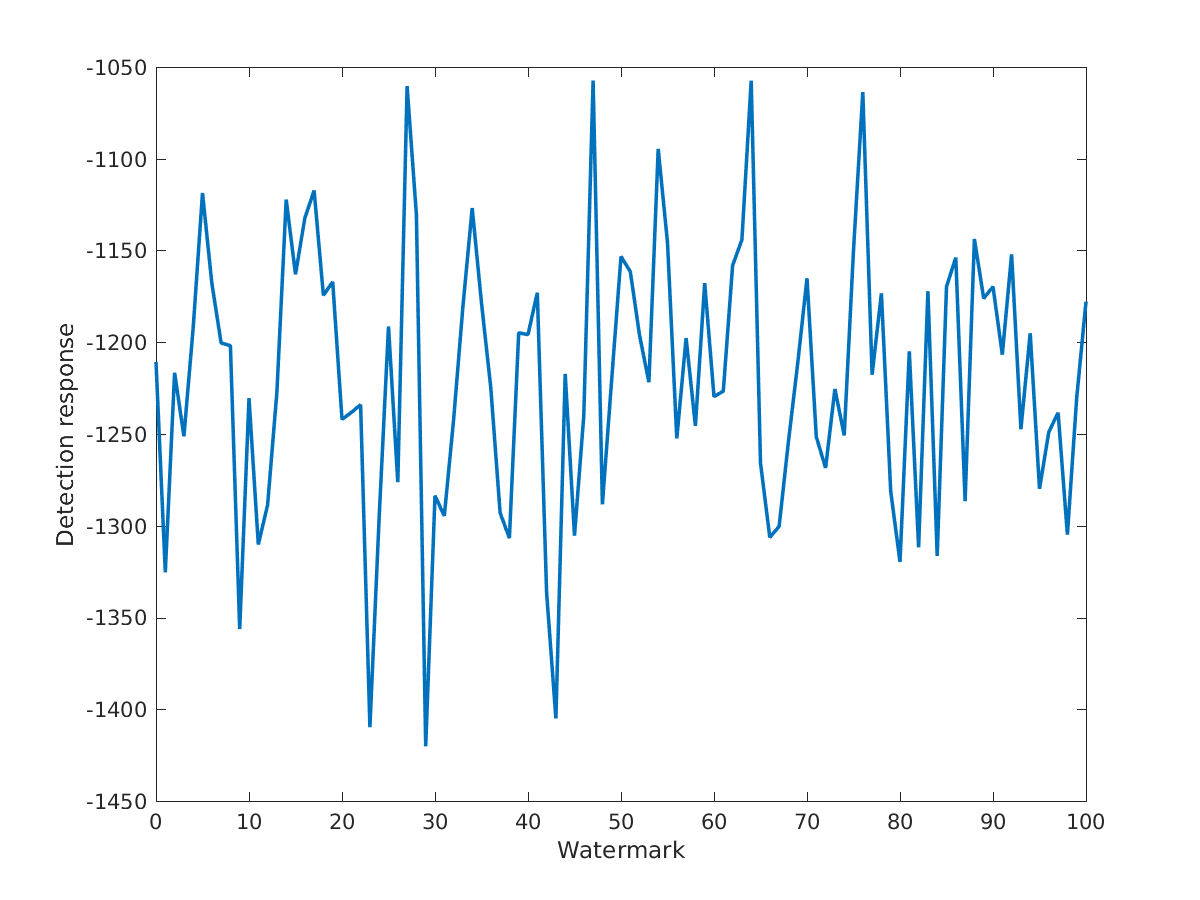
\includegraphics[width=1\textwidth]{./img/likelihood/correct_LikelihoodLr_NM.png}
           \caption{\small{detection on the right view}}
\label{fig:Lrnm}
    \end{subfigure}
    \caption{Detector response on the left and right views where the images hasn't been marked}
    \label{fig:Lnm}
\end{figure*}


Figures \ref{fig:Gl1}-\ref{fig:Gr3} show the response of the spatial watermarking detector, in terms of correlation value, to 100 randomly generated watermarks of which only one matches the reference watermark.\\

It is worth noting that the response due to the correct watermark is very much stronger with respect to the response in case of non watermarked video, suggesting that the algotithm has very low false positive (and false negative) response rate. This holds either for the left detection (figure \ref{fig:Ll03} and \ref{fig:Ll06}) and for the right detection(figure \ref{fig:Lr03} and \ref{fig:Lr06}). \newline Figures \ref{fig:Llnm} and  \ref{fig:Lrnm} prove that when the image under consideration doesn't contain the reference watermark the score array doesn't present any spikes.

\section{Robustness against compression attack}

In video analysis, compression helps to reduce resource usage, such as data storage space or transmission capacity.\newline This process is considered an attack since while bringing to a degradation of the image due to the compression ratio, it degradates also the watermark readability.\newline 
This problem can be coped improving the strenght of the embedded watermark, to resist the image degradation,while mantaining an acceptable trade-off between robustness and the perceptual impact of the watermark. \newline

Figures \ref{fig:03crf1}-\ref{fig:06crf25} show the degradation of the image due to compression and watermark power.


\begin{figure}[h!]
\centering
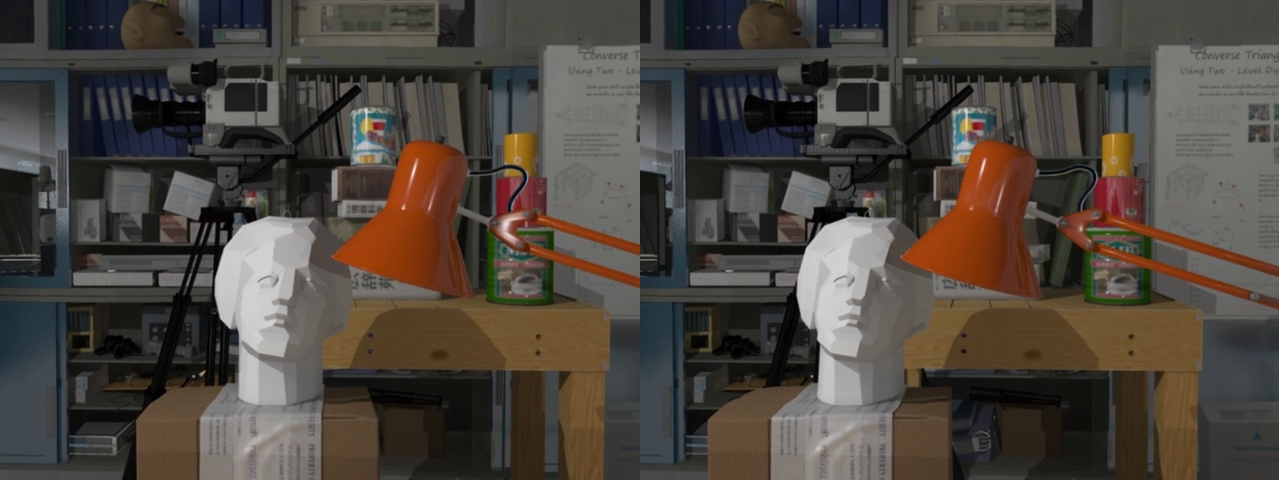
\includegraphics[width=0.9\textwidth]{./img/03_crf1_gt.png}
\caption{\small{Stereo image from video marked with power 0.3 and compressed with crf equal to 1 }}
\label{fig:03crf1}
\end{figure}
\begin{figure}[h!]
\centering
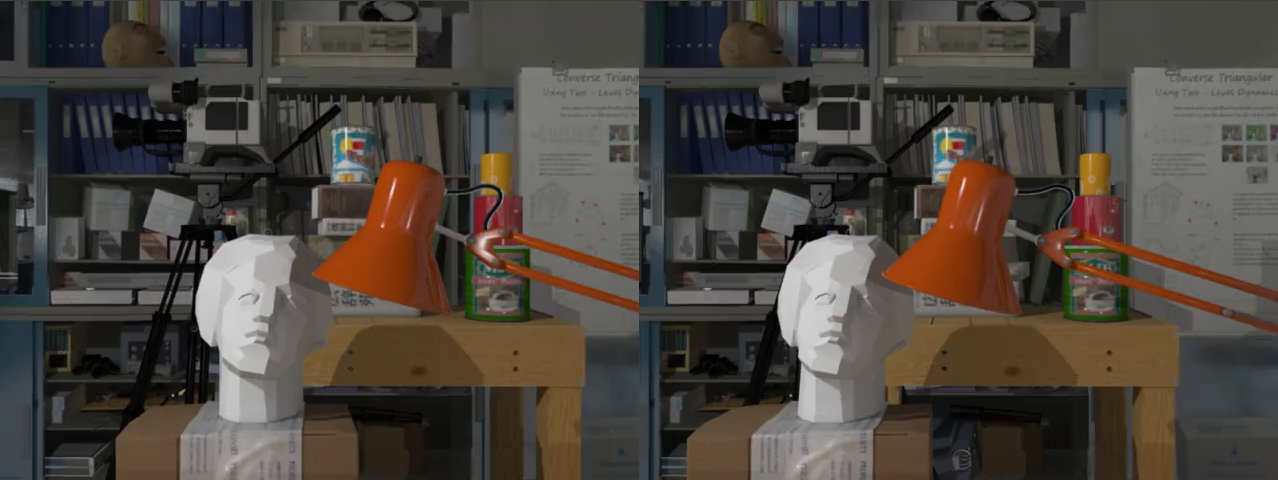
\includegraphics[width=0.9\textwidth]{./img/03_crf25_gt.png}
\caption{\small{Stereo image from video marked with power 0.3 and compressed with crf equal to 25 }}
\label{fig:03crf25}
\end{figure}
\begin{figure}[h!]
\centering
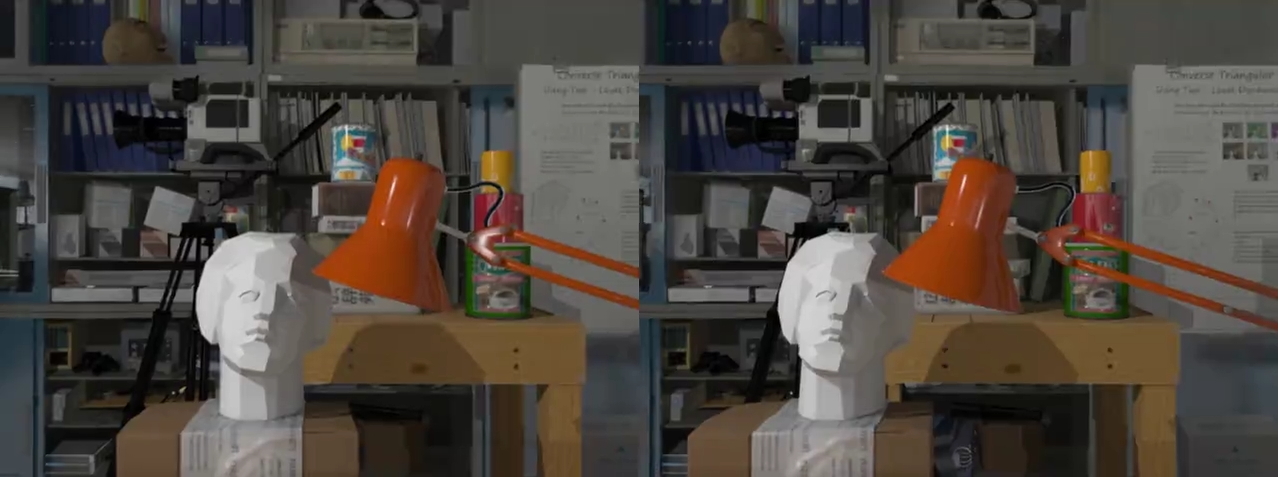
\includegraphics[width=0.9\textwidth]{./img/03_crf30_gt.png}
\caption{\small{stereo image from video marked with power 0.3 and compressed with crf equal to 30 }}
\label{fig:03crf30}
\end{figure}


\begin{figure}[h!]
\centering
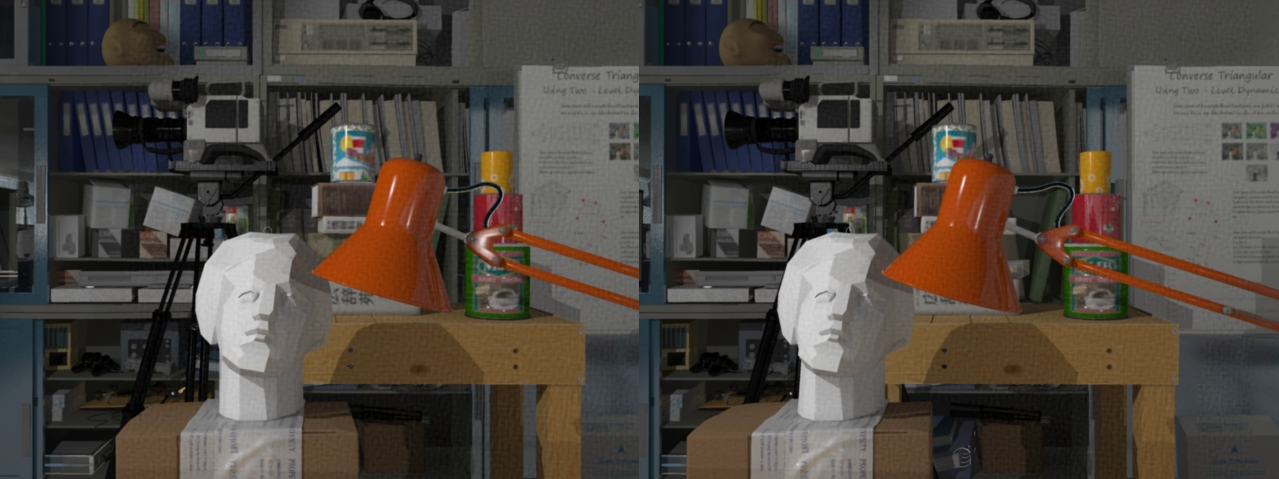
\includegraphics[width=0.9\textwidth]{./img/06_crf1_gt.png}
\caption{\small{Stereo image from video marked with power 0.6 and compressed with crf equal to 1 }}
\label{fig:06crf1}
\end{figure}
\begin{figure}[h!]
\centering
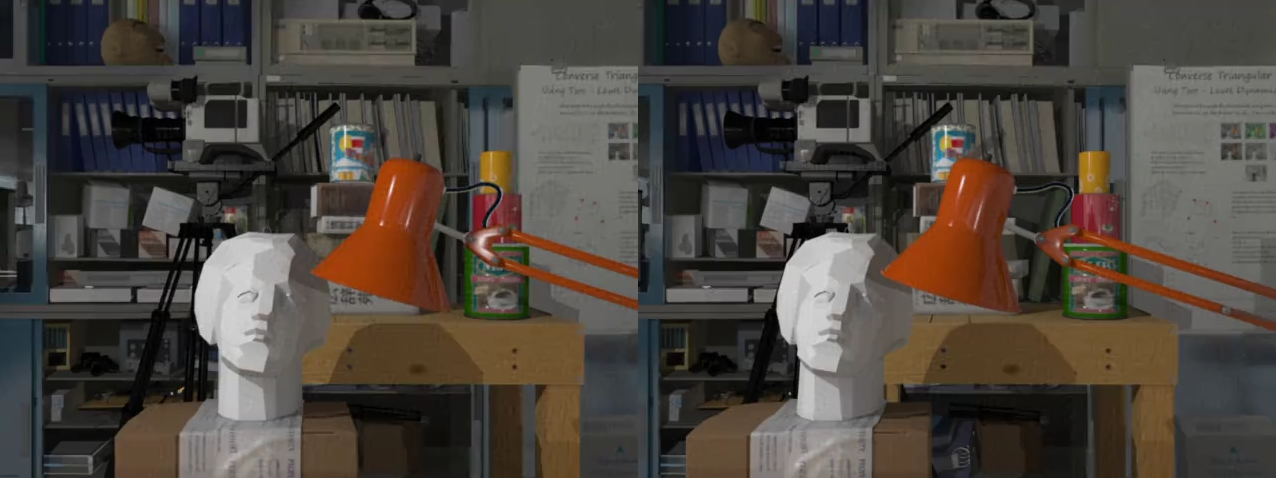
\includegraphics[width=0.9\textwidth]{./img/06_crf25_gt.png}
\caption{\small{Stereo image from video marked with power 0.6 and compressed with crf equal to 25 }}
\label{fig:06crf25}
\end{figure}
\begin{figure}[h!]
\centering
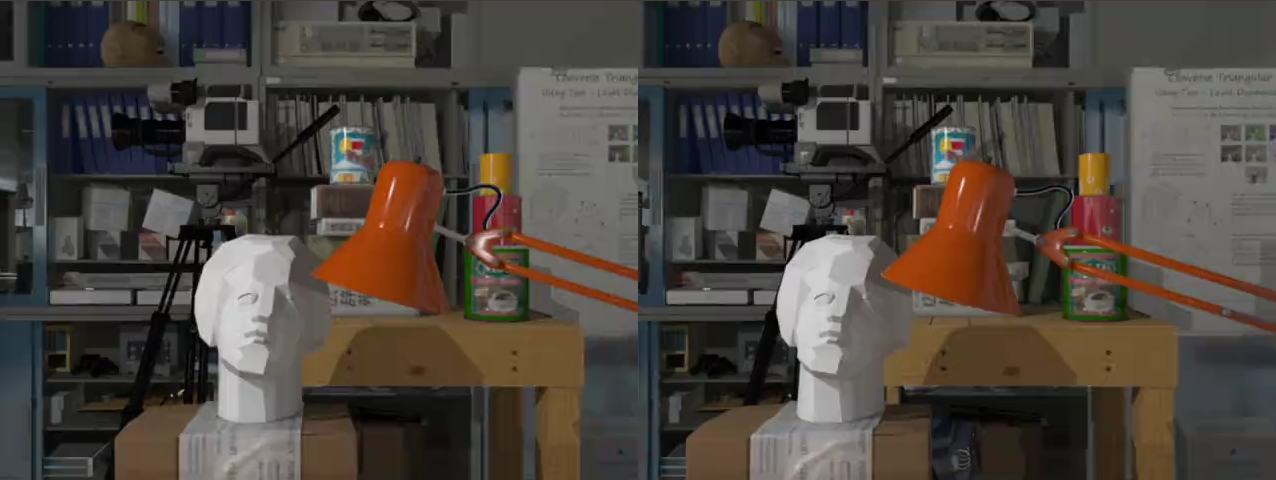
\includegraphics[width=0.9\textwidth]{./img/06_crf30_gt.png}
\caption{\small{stereo image from video marked with power 0.6 and compressed with crf equal to 30 }}
\label{fig:06crf30}
\end{figure}

\clearpage

In figures \ref{fig:03crf1}-\ref{fig:03crf30} the images has been marked with power equal to 0.3, we can see that this way the watermark does not affect the image and how the frames are degradated from the compression.

Yet in figures \ref{fig:06crf1}-\ref{fig:06crf30} it can be noted that when the power is equal to 0.6 the mark is perceptible and it become less visible the more the image is compressed. 


\subsection{Spatial watermarking robustness}

In spatial domain watermarking systems, the watermark is embedded directly in the pixel domain.\newline  Many of the spatial watermarking techniques provide simple and effective schemes for embedding an invisible watermark into an image, but are less robust to common attacks such as lossy compression.

The evaluation of this detection system has been studied through the ROC curve, which show the performance of a binary classifier system as its discrimination threshold is varied. The curve is created by plotting the true positive rate (TPR) against the false positive rate (FPR) at various threshold settings. The best possible prediction method would yield a point in the upper left corner or coordinate (0,1) of the ROC space, representing 100$\%$ sensitivity (no false negatives) and 100$\%$ specificity (no false positives). The (0,1) point is also called a perfect classification. A completely random guess would give a point along a diagonal line from the left bottom to the top right corners.

Figures \ref{fig:g1crf1}-\ref{fig:g3crf30} show the results for this experiment; each curve is the result of the study conducted on 30 marked frames when the positive score is assigned to : (i) the correlation value between the left view and the watermark, (ii) the correlation between the warped right view and the watermark, (iii) the correlation between the right view and the warped watermark.\\ The negative score is assigned to the correlation value produced by the right view and the reference watermark.

\begin{figure}[h!]
\centering
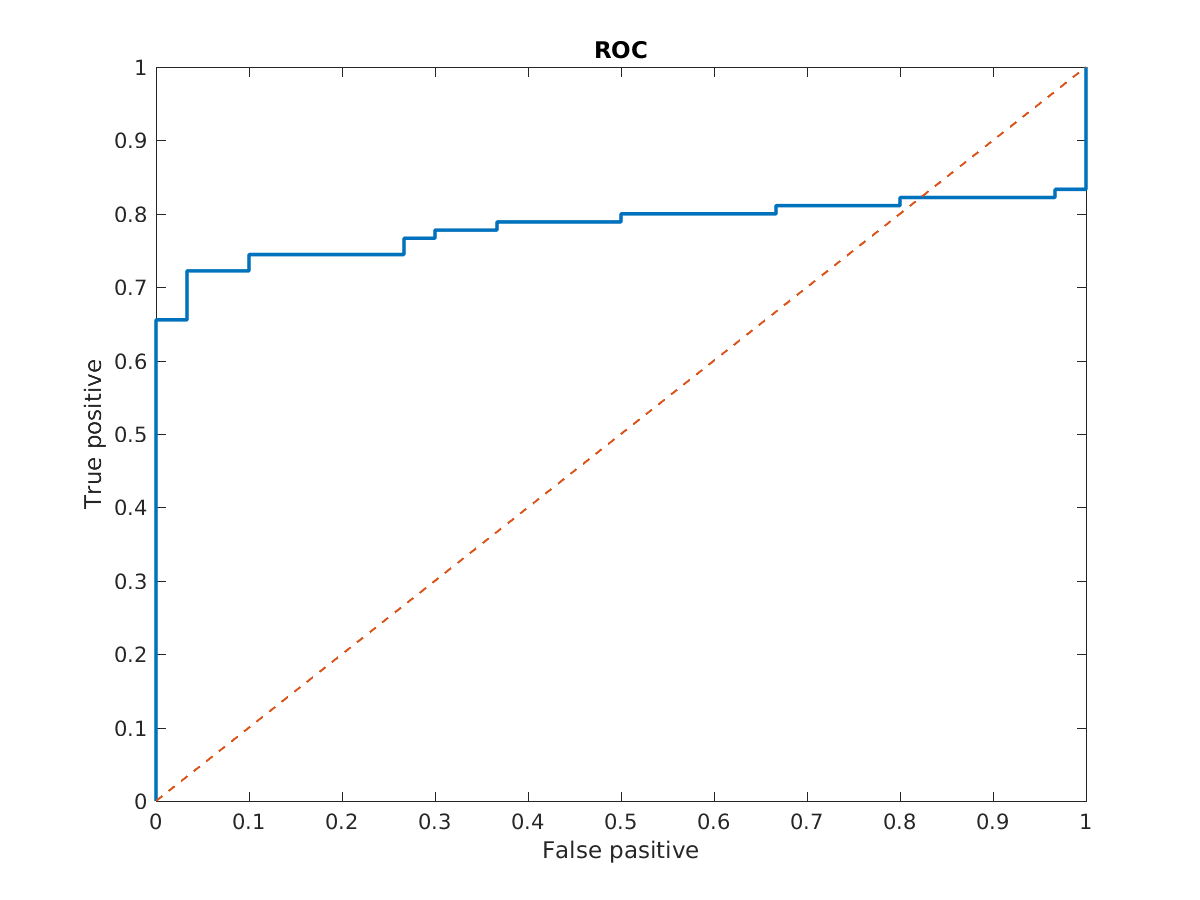
\includegraphics[width=0.6\textwidth]{./img/ROC/ROC_gauss_1_1.png}
\caption{\small{ROC curve of a spatial marked image with power equal to 1 and not compressed}}
\label{fig:g1crf1}
\end{figure}
\begin{figure}[h!]
\centering
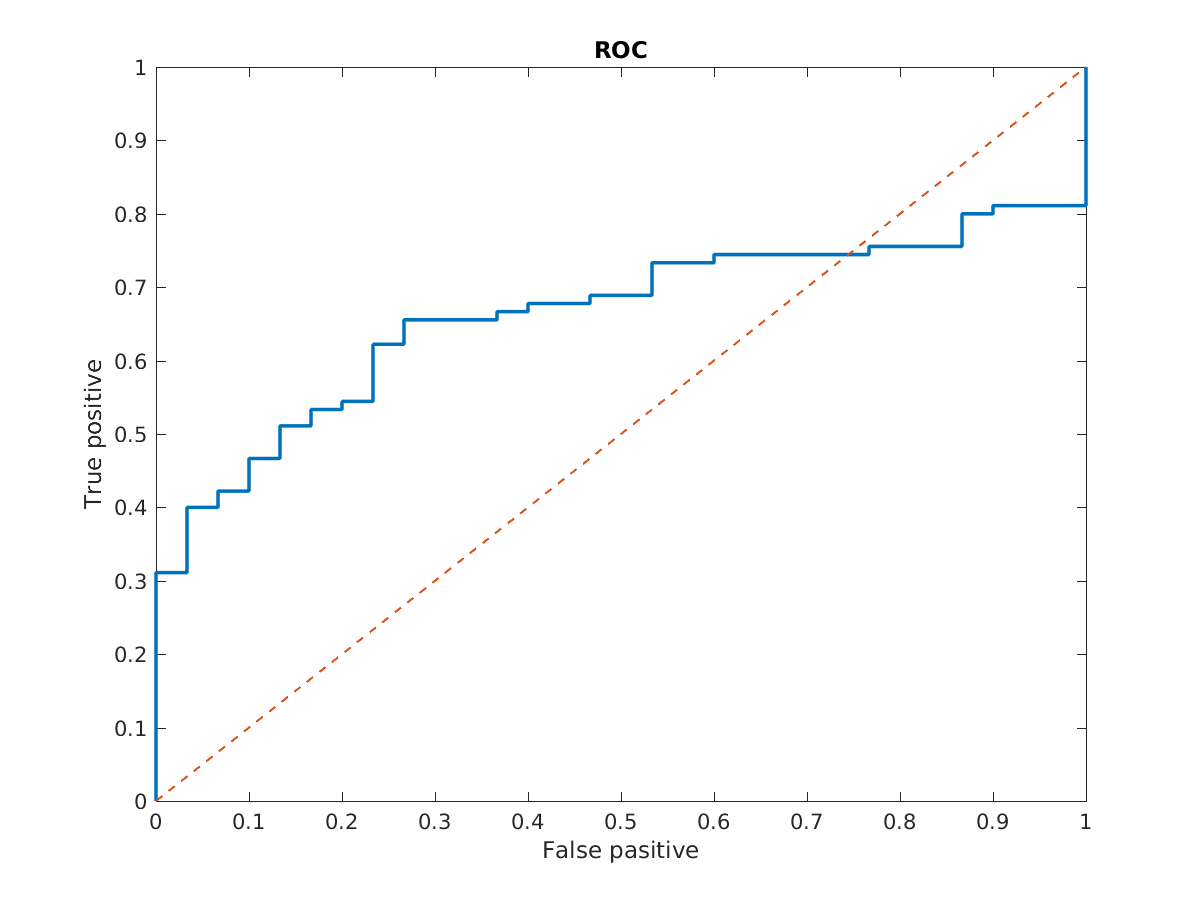
\includegraphics[width=0.6\textwidth]{./img/ROC/ROC_gauss_1_15.png}
\caption{\small{ROC curve of a spatial marked image with power equal to 1 and compressed with crf 15}}
\label{fig:g1crf15}
\end{figure}
\begin{figure}[h!]
\centering
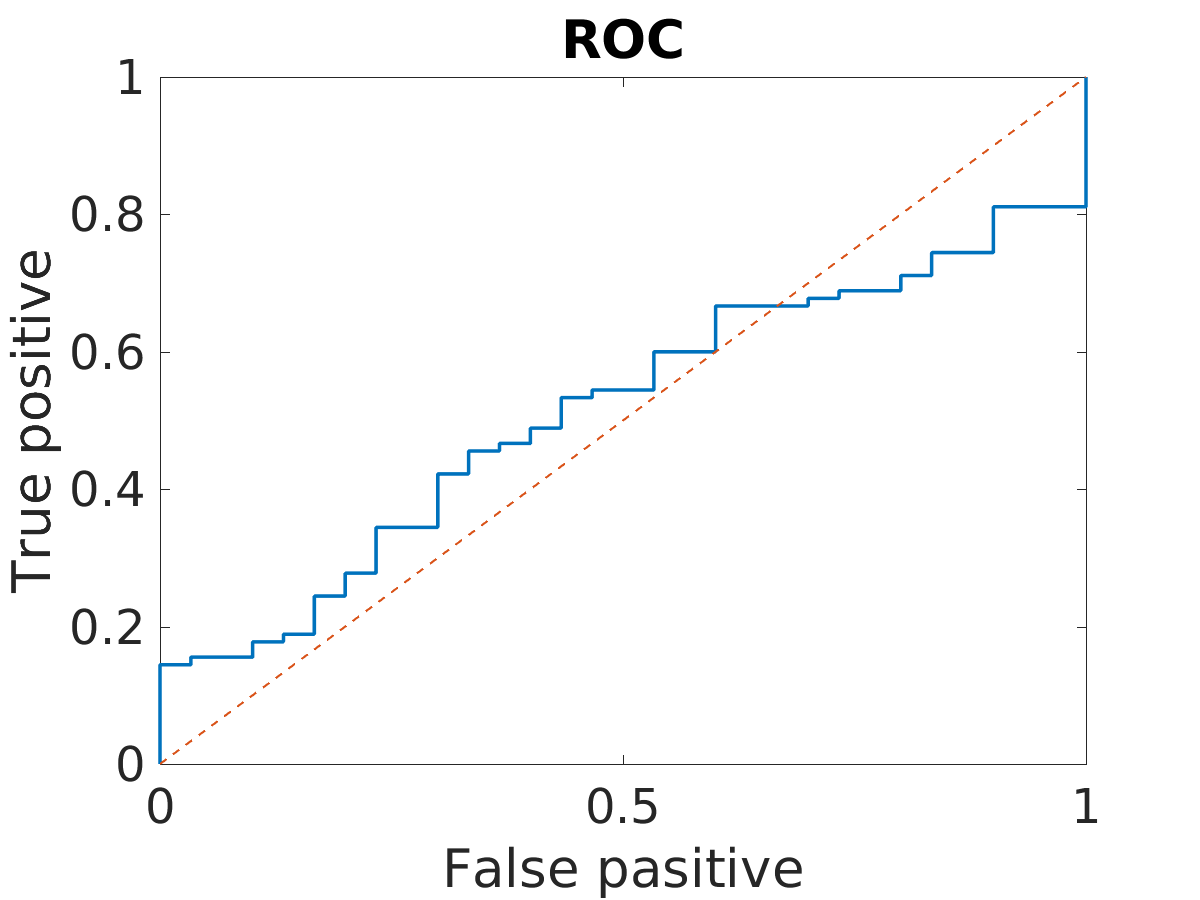
\includegraphics[width=0.6\textwidth]{./img/ROC/ROC_gauss_1_25.png}
\caption{\small{ROC curve of a spatial marked image with power equal to 1 and compressed with crf 25}}
\label{fig:g1crf25}
\end{figure}
\begin{figure}[h!]
\centering
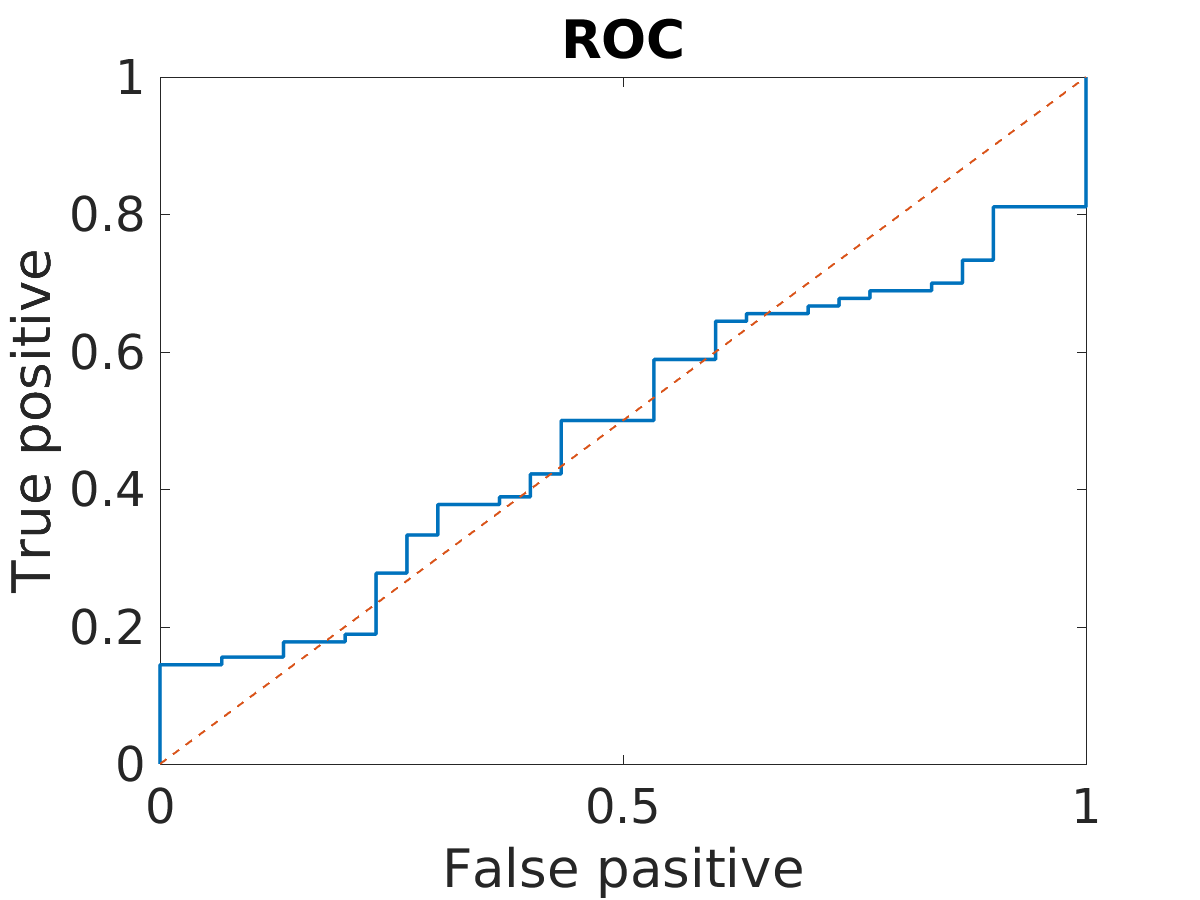
\includegraphics[width=0.6\textwidth]{./img/ROC/ROC_gauss_1_30.png}
\caption{\small{ROC curve of a spatial marked image with power equal to 1 and compressed with crf 30}}
\label{fig:g1crf30}
\end{figure}
\begin{figure}[h!]
\centering
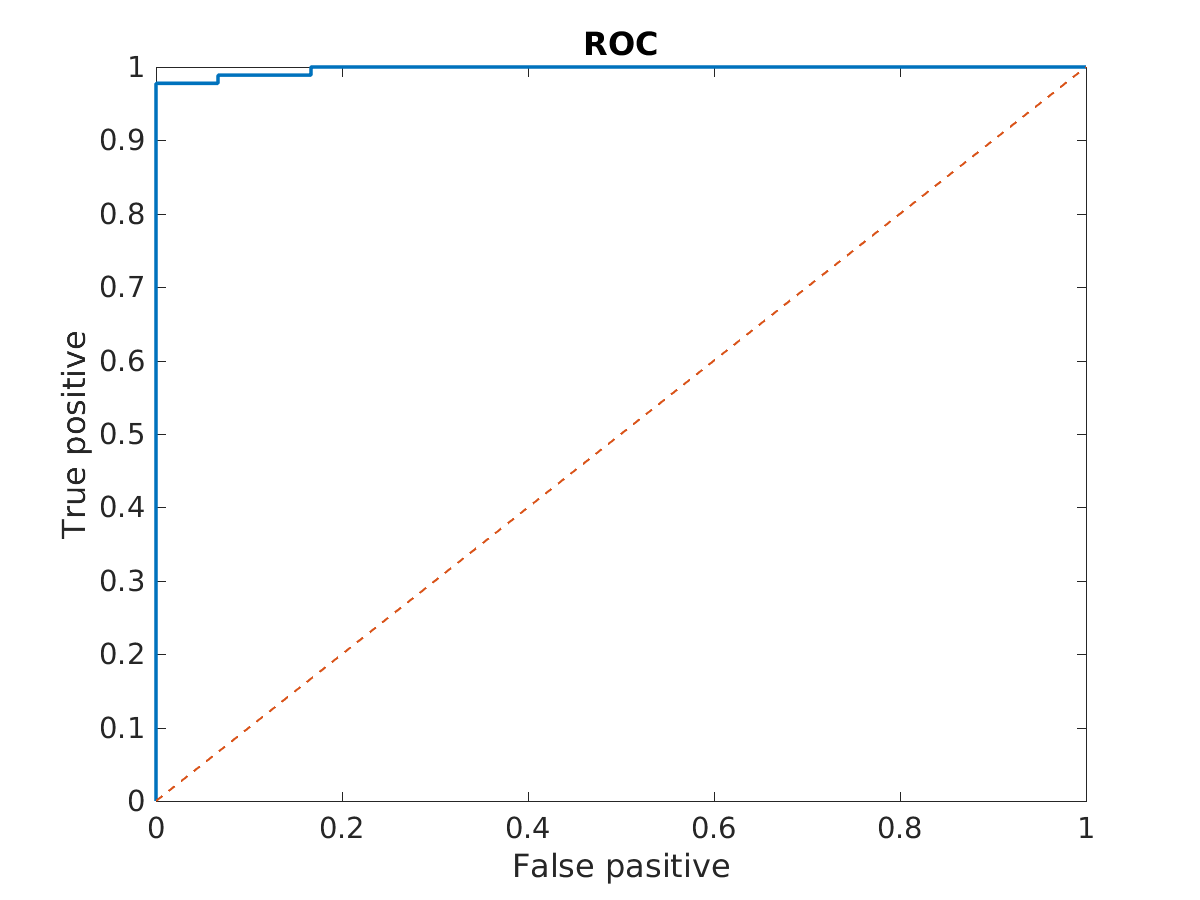
\includegraphics[width=0.6\textwidth]{./img/ROC/ROC_gauss_3_1.png}
\caption{\small{ROC curve of a spatial marked image with power equal to 3 and not compressed }}
\label{fig:g3crf1}
\end{figure}
\begin{figure}[h!]
\centering
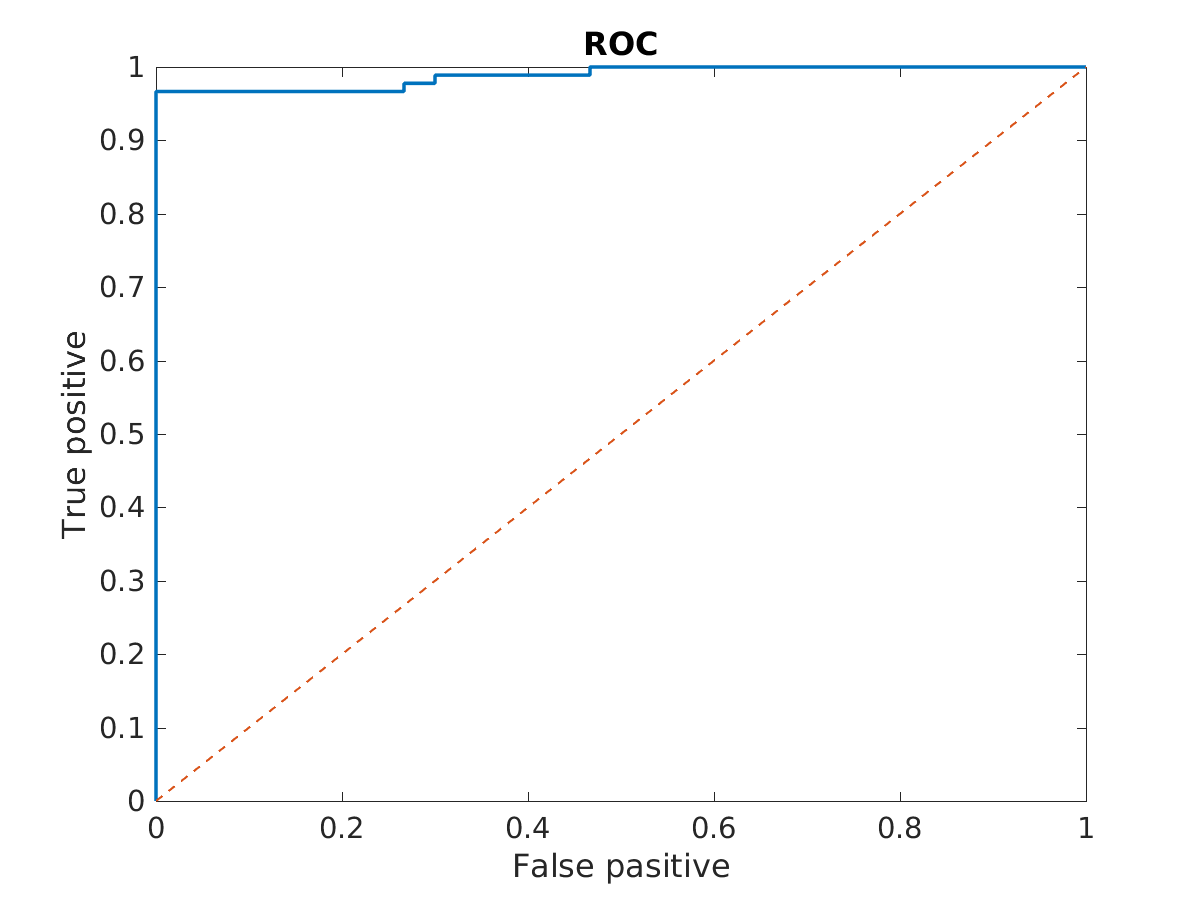
\includegraphics[width=0.6\textwidth]{./img/ROC/ROC_gauss_3_15.png}
\caption{\small{ROC curve of a spatial marked image with power equal to 3 and compressed with crf 15 }}
\label{fig:g3crf15}
\end{figure}
\begin{figure}[h!]
\centering
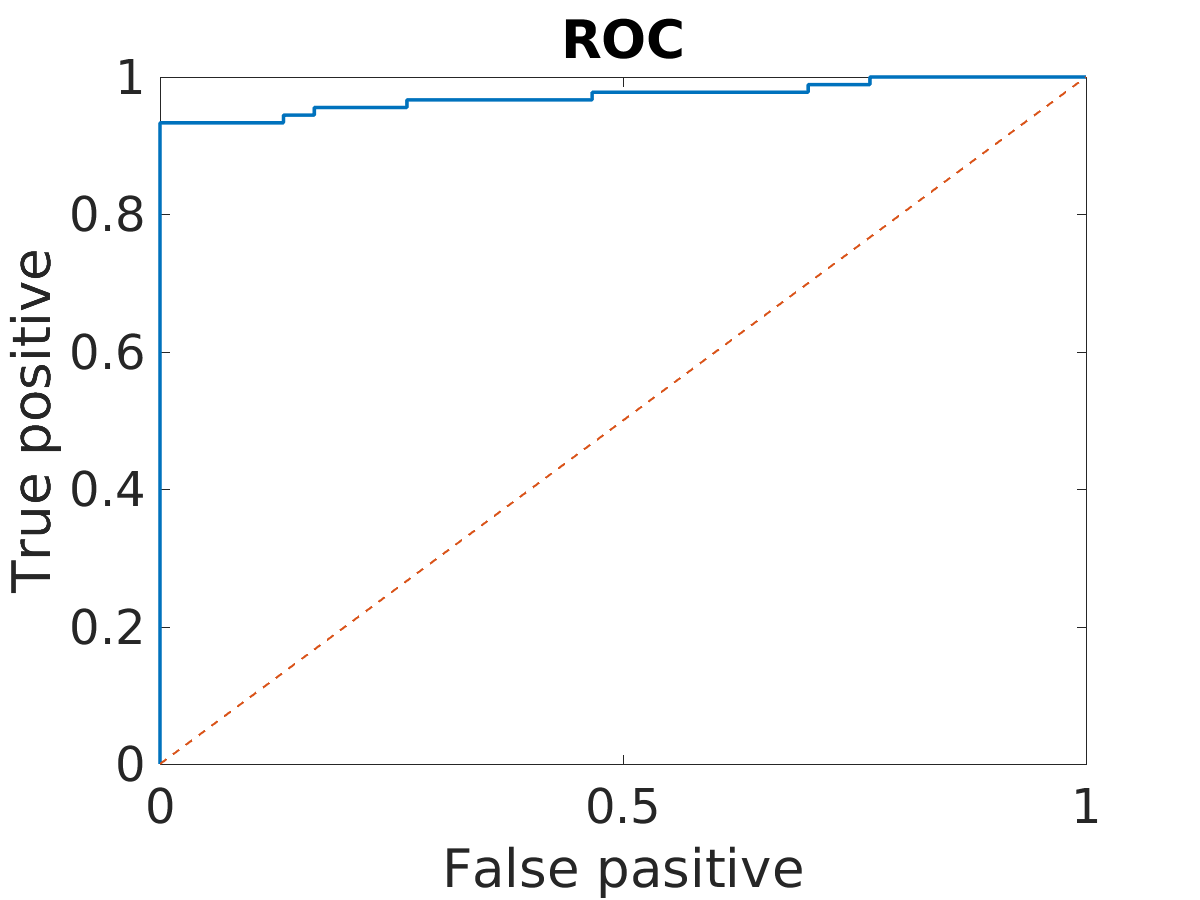
\includegraphics[width=0.6\textwidth]{./img/ROC/ROC_gauss_3_25.png}
\caption{\small{ROC curve of a spatial marked image with power equal to 3 and compressed with crf 25 }}
\label{fig:g3crf25}
\end{figure}
\begin{figure}[h!]
\centering
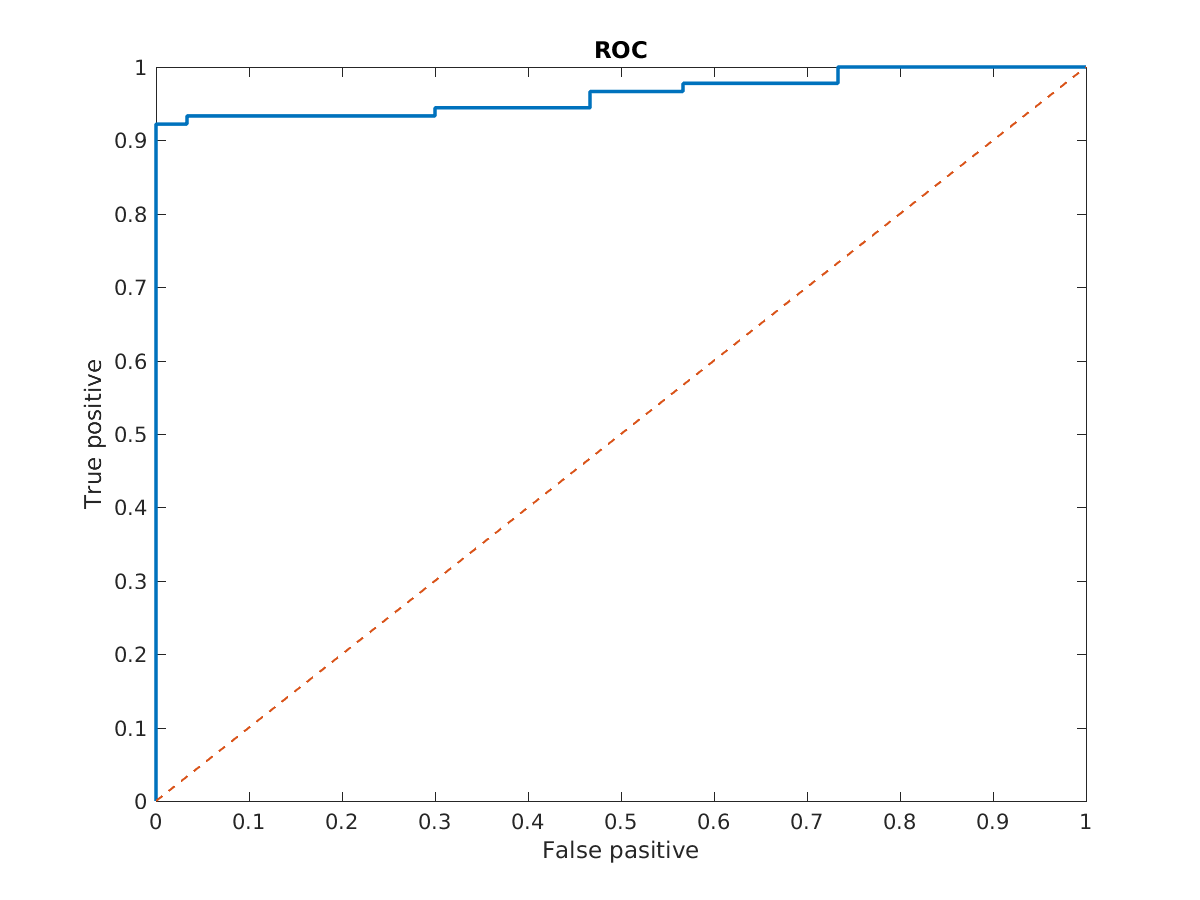
\includegraphics[width=0.6\textwidth]{./img/ROC/ROC_gauss_3_30.png}
\caption{\small{ROC curve of a spatial marked image with power equal to 3 and compressed with crf 30 }}
\label{fig:g3crf30}
\end{figure}
\clearpage

The ROC functions above reveal that the more the image is compressed the more the classification is a random guess, but when the mark is added with power equal to 3 the compression doesn't affect the detection process.

\subsection{DFT watermaking robustess}

Two studies are presented in this section: the first one concernes the power of the watermark needed in order to achieve robustness against different levels of compression; the latter focus on youtube, and tries to find the right power to achive robustness in a downloaded video.
 
Tables \ref{tab:compgt}-\ref{tab:compkz} shows how the algorithm manage to find the watermark in a compressed video, in particular it is shown in how many stereo frame the mark is detected in both left and right view, and the total of correct detection on the left view and right view separately. The first table shows the results when the algorithm is used with the ground truth disparity, the second when using graph cuts.

\clearpage

\begin{table}[htbp]

 \begin{center}
 \scalebox{0.9}{ 
 \begin{tabular}{c|c|c c c }
 \hline\hline
 \multirow{1}{2.5cm}{\textbf{power}}&\multirow{1}{4cm}{\textbf{compression level}} & \multicolumn{1}{c}{\textbf{both}} & \multicolumn{1}{c}{\textbf{left}} & \multicolumn{1}{c}{\textbf{right}}\\ \hline
 
0.3 & 1 & 30 & 30 & 30 \\
0.3 & 15 & 30 & 30 & 30 \\
0.3 & 25 & 10 & 15 & 10 \\
0.3 & 30 & 1 & 2 & 1 \\
0.5 & 1 & 30 & 30 & 30 \\
0.5 & 15 & 30 & 30 & 30 \\
0.5 & 25 & 23 & 25 & 24 \\
0.5 & 30 & 10 & 14 & 10 \\
0.6 & 1 & 30 & 30 & 30 \\
0.6 & 15 & 30 & 30 & 30 \\
0.6 & 25 & 28 & 28 & 28 \\
0.6 & 30 & 16 & 18 & 16 \\
           
 \hline
 \end{tabular}
 }
 \caption{ detection table when ground truth disparity is used  \label{tab:compgt}}
 \end{center}
 \end{table}

\begin{table}[htbp]

 \begin{center}
 \scalebox{0.9}{ 
 \begin{tabular}{c|c|c c c }
 \hline\hline
 \multirow{1}{2.5cm}{\textbf{power}}&\multirow{1}{4cm}{\textbf{compression level}} & \multicolumn{1}{c}{\textbf{both}} & \multicolumn{1}{c}{\textbf{left}} & \multicolumn{1}{c}{\textbf{right}}\\ \hline
 
 0.3 & 1 & 30 & 30 & 30 \\
 0.3 & 15 & 29 & 30 & 29 \\
 0.3 & 25 & 11 & 12 & 11 \\
 0.3 & 30 & 2 & 3 & 2 \\
 0.5 & 1 & 30 & 30 & 30 \\
 0.5 & 15 & 30 & 30 & 30 \\
 0.5 & 25 & 24 & 26 & 24 \\
 0.5 & 30 & 9 & 11 & 9 \\
 0.6 & 1 & 30 & 30 & 30 \\
 0.6 & 15 & 30 & 30 & 30 \\
 0.6 & 25 & 26 & 27 & 27 \\
 0.6 & 30 & 15 & 19 & 15 \\
           
 \hline
 \end{tabular}
 }
 \caption{Detection table when graph cuts disparity is used \label{tab:compkz}}
 \end{center}
 \end{table}
 
One can notice that, at a global level, detection statistics gradually degrade with the compression ratio. The embedded watermark becomes hardly detectable at the crudest compression levels even with if embedded with a strong power. \newline From the results emerges that when the watermark power is grater than or equal to 0.5 the detection supports a compression level of 25 with good statistics.

Figures \ref{fig:03yt}-\ref{fig:08yt} show how the uploading and the subsequential download of a non compressed video on youtube degradates the image.\newline
 
\begin{figure}[h!]
\centering
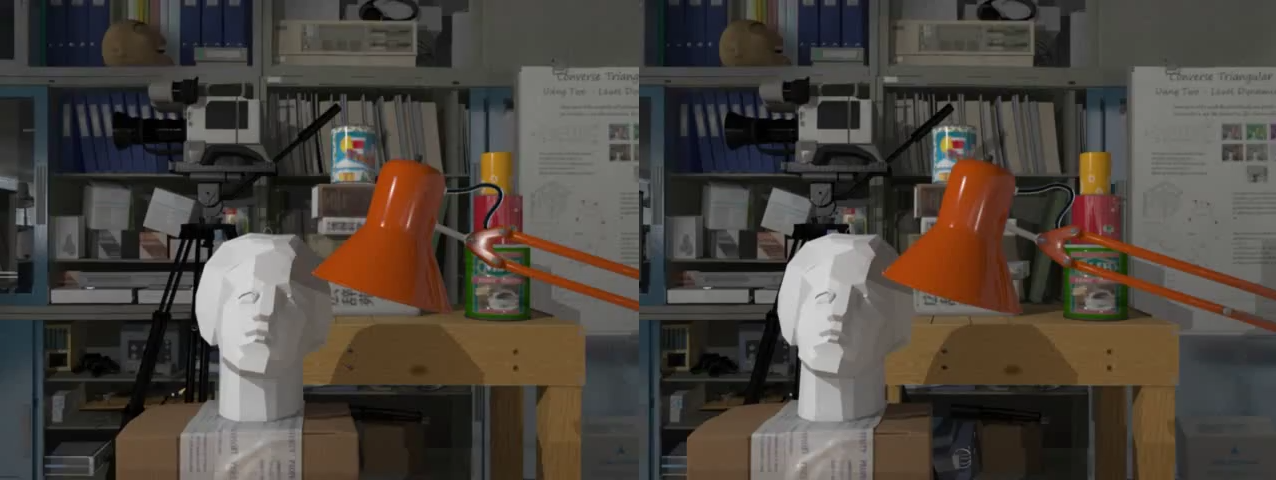
\includegraphics[width=0.9\textwidth]{./img/yt_03_gt.png}
\caption{\small{Stereo image from video uploaded with power equal to 0.3 }}
\label{fig:03yt}
\end{figure}
\begin{figure}[h!]
\centering
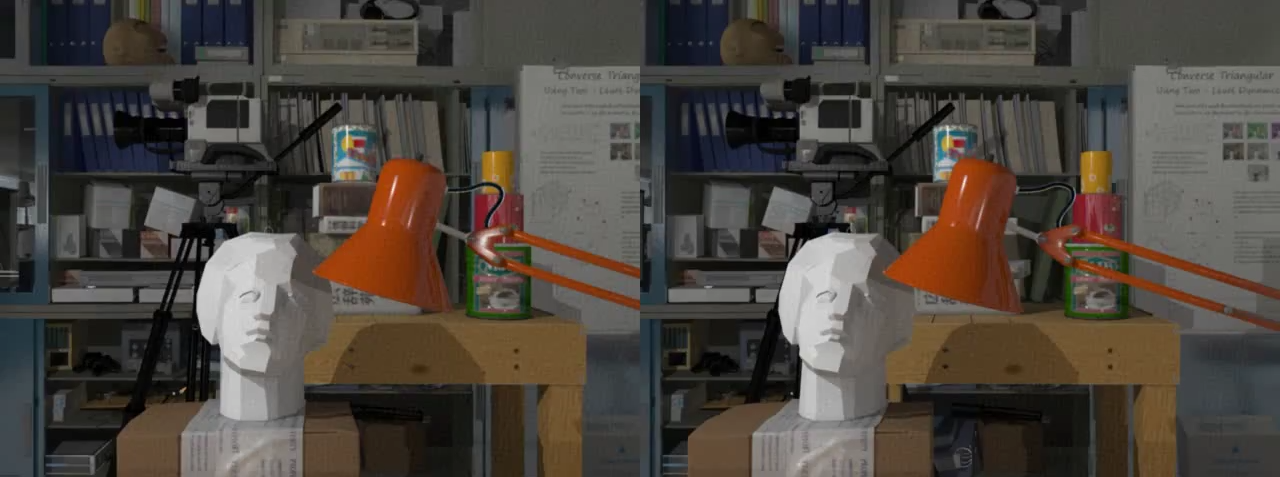
\includegraphics[width=0.9\textwidth]{./img/yt_06_gt.png}
\caption{\small{Stereo image from video uploaded with power equal to 0.6 }}
\label{fig:06yt}
\end{figure}
\begin{figure}[h!]
\centering
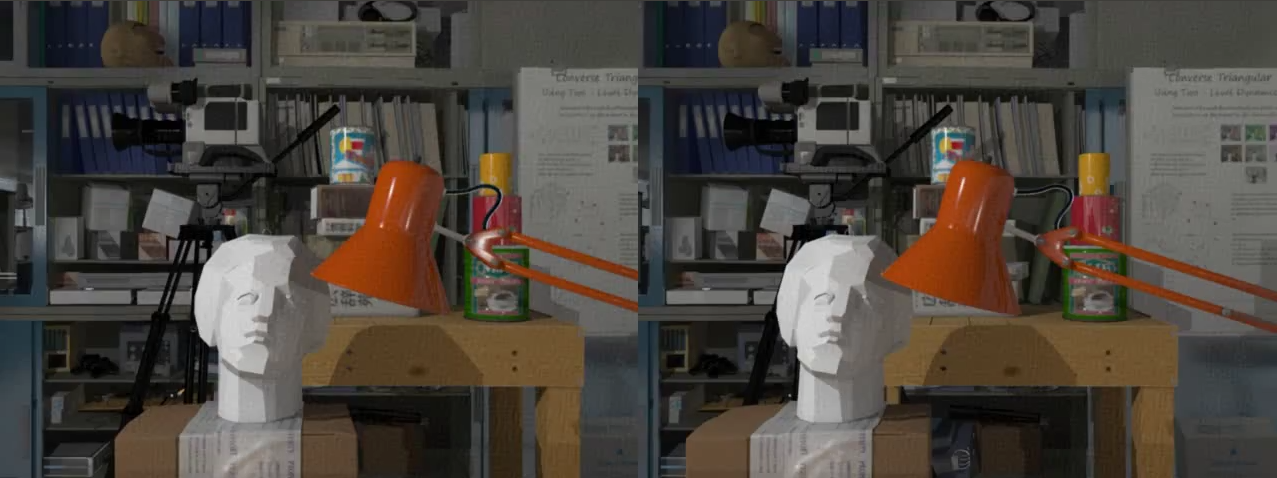
\includegraphics[width=0.9\textwidth]{./img/yt_07_gt.png}
\caption{\small{Stereo image from video uploaded with power equal to 0.7 }}
\label{fig:07yt}
\end{figure}
\begin{figure}[h!]
\centering
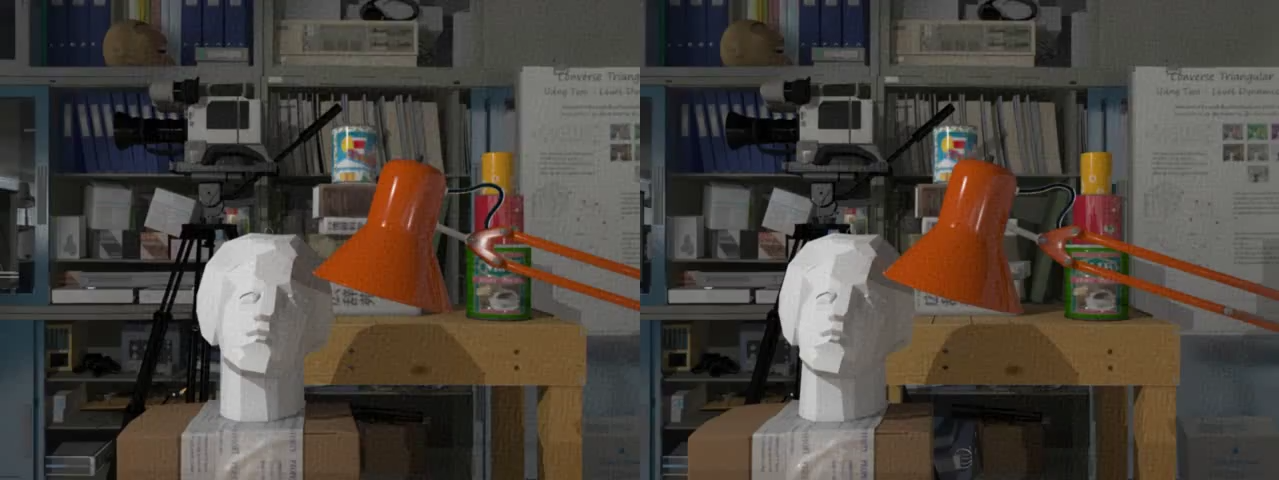
\includegraphics[width=0.9\textwidth]{./img/yt_08_gt.png}
\caption{\small{Stereo image from video uploaded with power equal to 0.8 }}
\label{fig:08yt}
\end{figure}
\clearpage

From Figures \ref{fig:03yt}-\ref{fig:08yt} it can be noticed that as a consequence of the image degradation the watermark become less perceptible even when inserted with a high power. 

Tables \ref{tab:ytgt}-\ref{tab:ytkz} show how a video uploaded on youtube and subsequentially downloaded can preserve the watermark, respectively when the watermark is inserted with the ground truth disparity and with graph cuts.\newline
 
 
 \begin{table}[htbp]

  \begin{center}
  \scalebox{0.9}{ 
  \begin{tabular}{c|c c c }
  \hline\hline
  \multirow{1}{2.5cm}{\textbf{power}} & \multicolumn{1}{c}{\textbf{both}} & \multicolumn{1}{c}{\textbf{left}} & \multicolumn{1}{c}{\textbf{right}}\\ \hline
 0.3 & 1 & 1 & 0\\
 0.6 & 9 & 10 & 9\\
 0.7 & 12& 14 & 12\\
  \hline
  \end{tabular}
  }
  \caption{Detection statistic for a downloaded video marked with ground truth disparity\label{tab:ytgt}}
  \end{center}
  \end{table}
 
\begin{table}[htbp]
 
 \begin{center}
 \scalebox{0.9}{ 
 \begin{tabular}{c|c c c }
 \hline\hline
 \multirow{1}{2.5cm}{\textbf{power}} & \multicolumn{1}{c}{\textbf{both}} & \multicolumn{1}{c}{\textbf{left}} & \multicolumn{1}{c}{\textbf{right}}\\ \hline

0.3& 1 & 1& 0\\
0.5& 6 & 7& 6\\
0.6& 11 & 11 & 0\\
 \hline
 \end{tabular}
 }
 \caption{Detection statistic for a downloaded video marked with graph cuts disparity\label{tab:ytkz}}
 \end{center}
 \end{table}
 
\subsection{PSNR test}
To validate this results the average PSNR value has been computed between original and compressed  stereoscopic videos at diffent compression levels.\\
PSNR is the ratio between the maximum possible power of a signal and the power of corrupting noise that affects the fidelity of its representation; it is usually expressed in terms of the logarithmic decibel scale (dB) and typical values for the PSNR in video compression and watermarking are between 30 and 50 dB.
The results of this study are shown in Table \ref{tab:psnr}: PSNR value decreases with the increment of the compression level. This implicates a decrement of the true positive rate after compression due to the image degradation as shown in Tables \ref{tab:compgt}-\ref{tab:compkz} and \ref{tab:ytgt}-\ref{tab:ytkz}.\\
\begin{table}[htbp]
\begin{center}
\scalebox{0.9}{ 
\begin{tabularx}{0.7\textwidth}{>{\centering\arraybackslash}X>{\centering\arraybackslash}X}
\hline \hline
Compression Level(CRF) & PSNR(dB) \\ \hline
15 		    & 46.0194 \\
25 		    & 40.4861 \\
YT 		    & 38.2039 \\
30 		    & 37.5587 \\
\hline 
\end{tabularx}
 }
\caption{\small{Average PSNR values between original video and compressed videos at different compression levels. The acronym YT stands for YouTube compression level, whose value is between 25 and 30 as the PSNR results show.} \label{tab:psnr}}
\end{center}
\end{table}

\section{Robustness to View Synthesis}
 
In a second batch of experiments, we analyzed the impact of virtual view synthesis on the detection performances of our watermarking system.

View synthesis can be viewed as the interpolation of a virtual view from two reference views. The reference views are essentially warped to the virtual viewpoint based on depth information and the intrinsic and extrinsic camera parameters and merged together.\newline
The view synthesis process using depth itself may destroy the watermark, as a result, to achieve robustness against this process, it is important to design the watermarks inserted in the left and right views so that they nicely overlap after the warping operation and thereby complement each other rather than cancel one another. The same 3D point should always carry the same watermark sample wherever it is projected in a view; hence we used a disparity-coherent technique.

To conduct these experiments, we generated a number of intermediate synthetic views (figures \ref{fig:synt1/4}-\ref{fig:synt3/4}), equally spaced apart between the left (reference) view and the right one, using the code in \cite{VS}.\newline


\begin{figure}[h!]
\centering
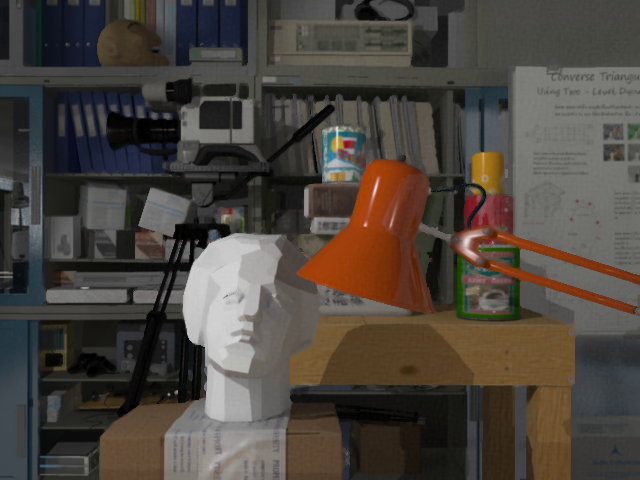
\includegraphics[width=0.5\textwidth]{./img/synth_view1_25.png}
\caption{\small{Synthetized view at distance 1/4 of the baseline from the left image }}
\label{fig:synt1/4}
\end{figure}
\begin{figure}[h!]
\centering
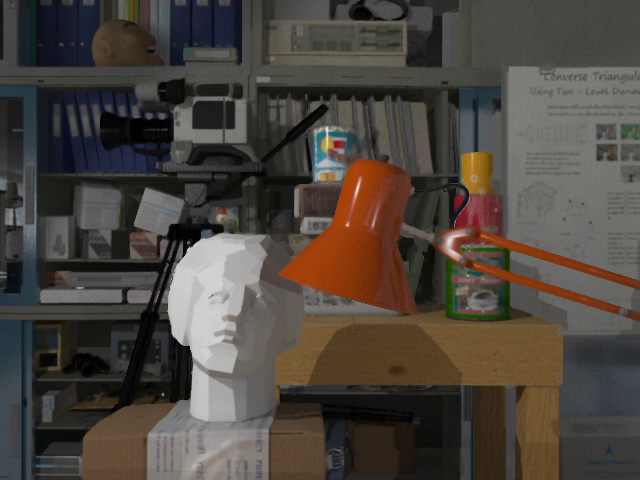
\includegraphics[width=0.5\textwidth]{./img/synth_view1_50.png}
\caption{\small{Synthetized view at distance 1/2 of the baseline from the left image }}
\label{fig:synt1/2}
\end{figure}
\begin{figure}[h!]
\centering
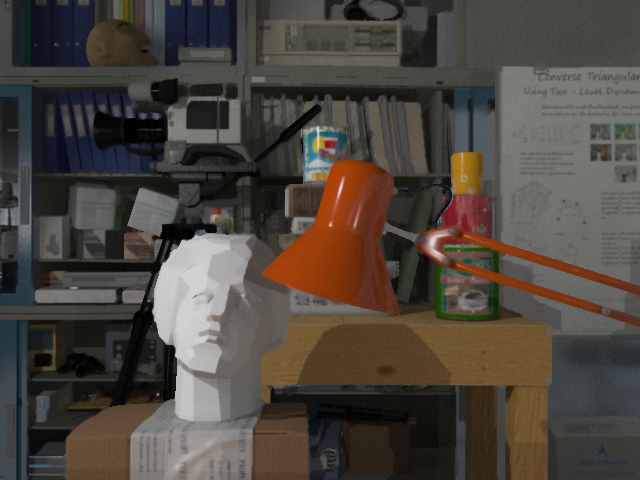
\includegraphics[width=0.5\textwidth]{./img/synth_view1_75.png}
\caption{\small{Synthetized view at distance 3/4 of the baseline from the left image }}
\label{fig:synt3/4}
\end{figure}

The Table \ref{tab:syntDFT} contains the results for the frequency marking: the first column is the distance between the left view and the synthetized one, in terms of fraction of the baseline, then its show in how many synthetized images the mark is detected.

\begin{table}[htbp]

 \begin{center}
 \scalebox{0.9}{ 
 \begin{tabular}{c|c c c }
 \hline\hline
 \multirow{1}{2.5cm}{\textbf{position}} & \multicolumn{1}{c}{\textbf{both}} & \multicolumn{1}{c}{\textbf{left}} & \multicolumn{1}{c}{\textbf{right}}\\ \hline

1/2 & 30& 0& 0\\
1/4 & 30& 0& 0\\
3/4 & 29 & 1 & 0\\
 \hline
 \end{tabular}
 }
 \caption{Detection in the syntetized views \label{tab:syntDFT}}
 \end{center}
 \end{table}
 
  
The same study is proposed for the spatial marking: from a video marked with additive gaussian noise have been generated three synthetized views for each pair of marked frames, respectively one in the middle and the other two at 1/4 and 3/4 of distance from the left.\newline The ROC curves in figures \ref{fig:g1vs25}-\ref{fig:g3vs75}  show the results for the different intermediate synthetic views.\newline 
\begin{figure}[h!]
\centering
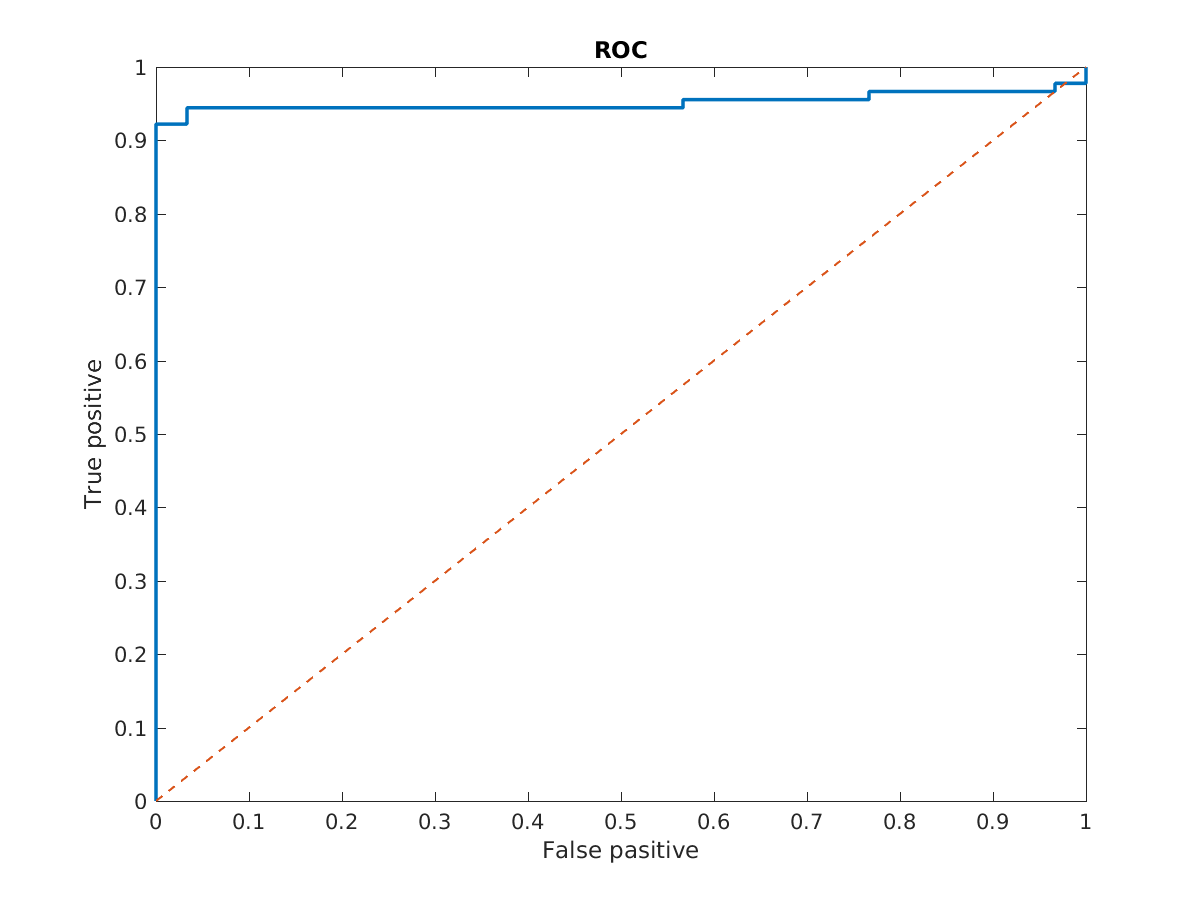
\includegraphics[width=0.6\textwidth]{./img/ROC/ROC_gauss_synt_1_25.png}
\caption{\small{ROC curve of a synthetic view created at distance equal to baseline/4 marked with power equal to 1 }}
\label{fig:g1vs25}
\end{figure}
\begin{figure}[h!]
\centering
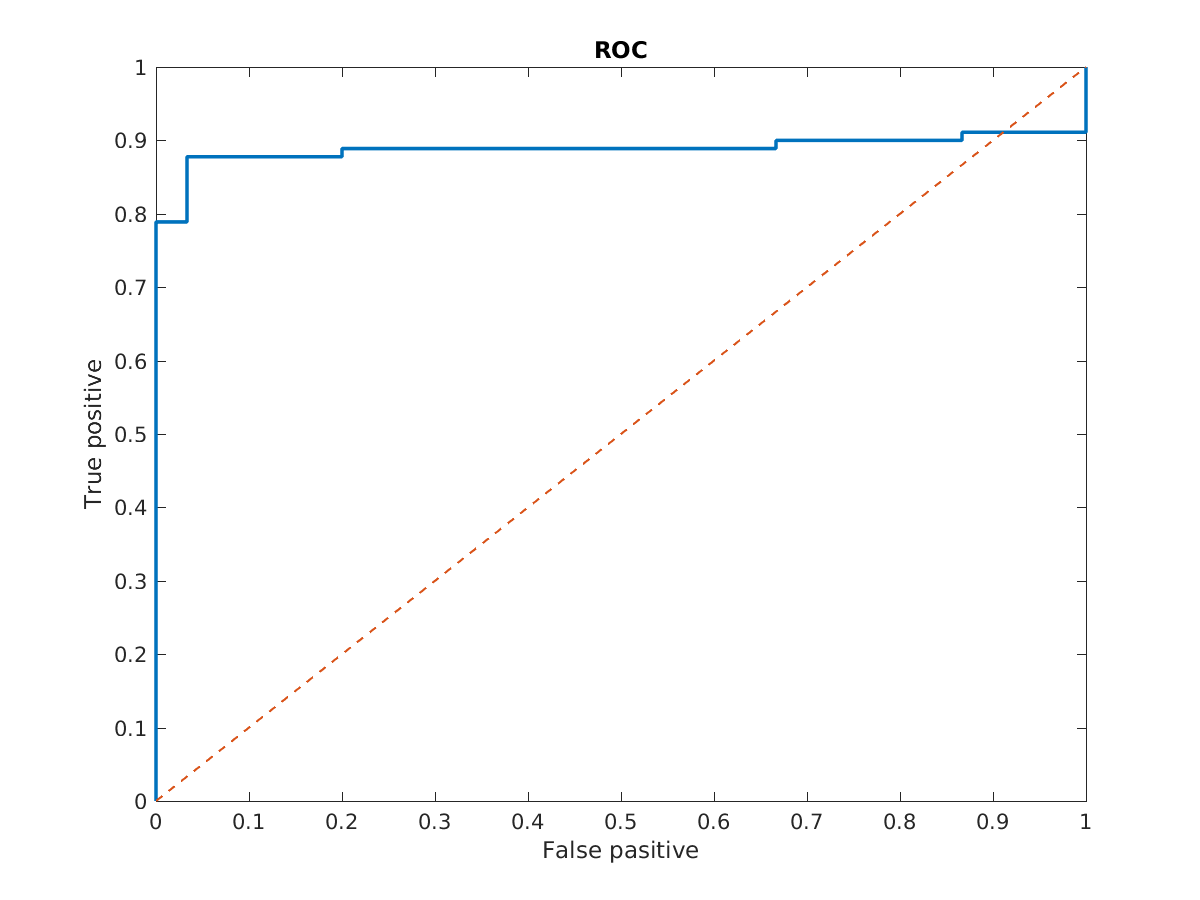
\includegraphics[width=0.6\textwidth]{./img/ROC/ROC_gauss_synt_1_50.png}
\caption{\small{ROC curve of a synthetic view created at distance equal to baseline/2 marked with power equal to 1 }}
\label{fig:g1vs50}
\end{figure}
\begin{figure}[h!]
\centering
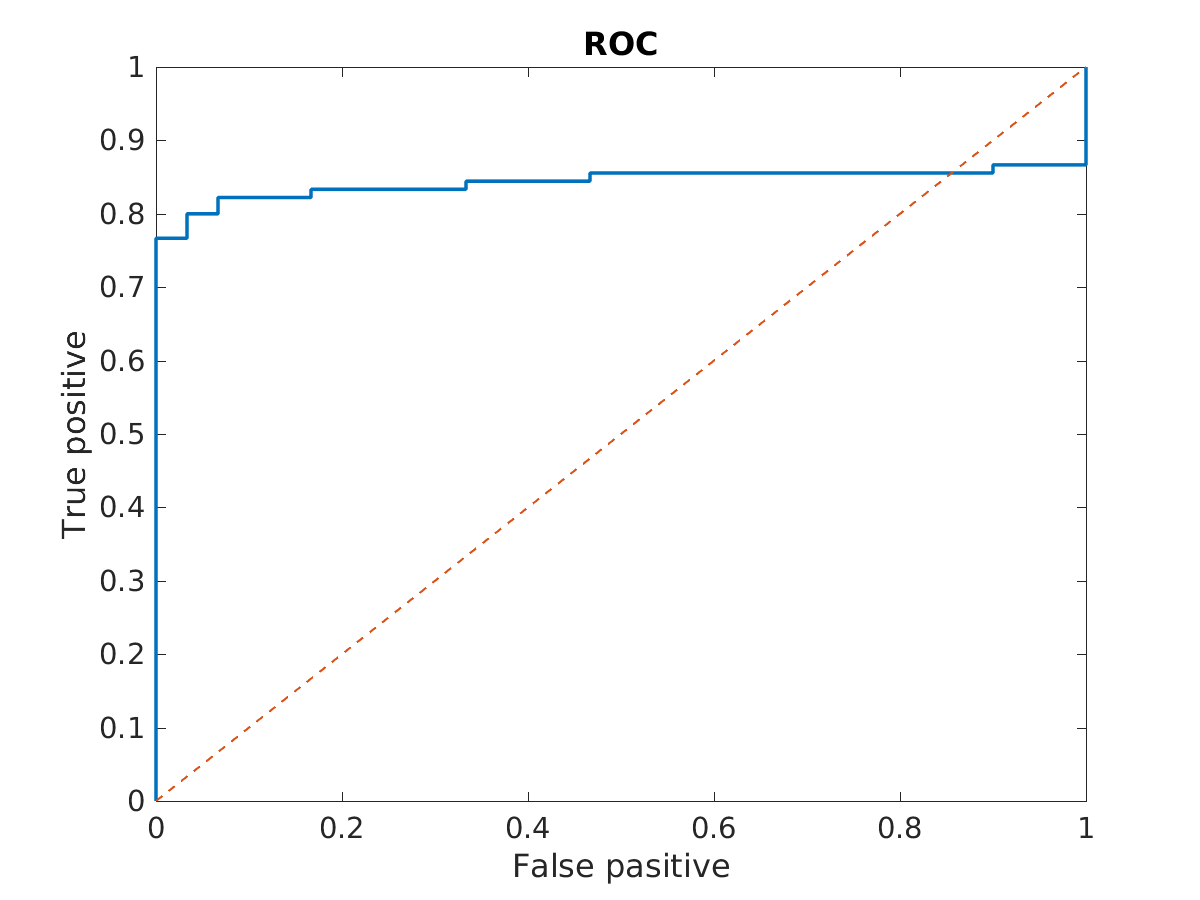
\includegraphics[width=0.6\textwidth]{./img/ROC/ROC_gauss_synt_1_75.png}
\caption{\small{ROC curve of a synthetic view created at distance equal to baseline*3/4 marked with power equal to 1 }}
\label{fig:g1vs75}
\end{figure}
\begin{figure}[h!]
\centering
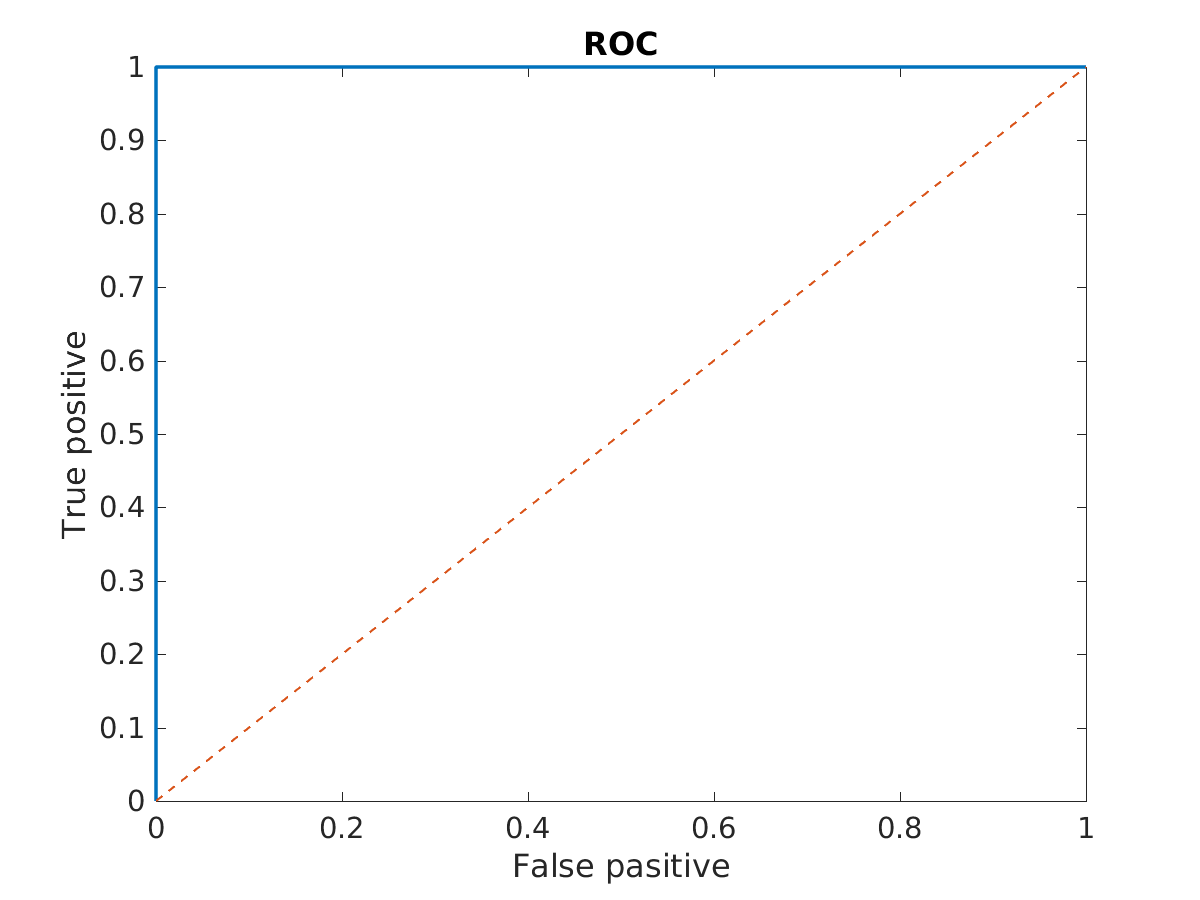
\includegraphics[width=0.6\textwidth]{./img/ROC/ROC_gauss_synt_3_25.png}
\caption{\small{ROC curve of a synthetic view created at distance equal to baseline/4 marked with power equal to 3 }}
\label{fig:g3vs25}
\end{figure}
\begin{figure}[h!]
\centering
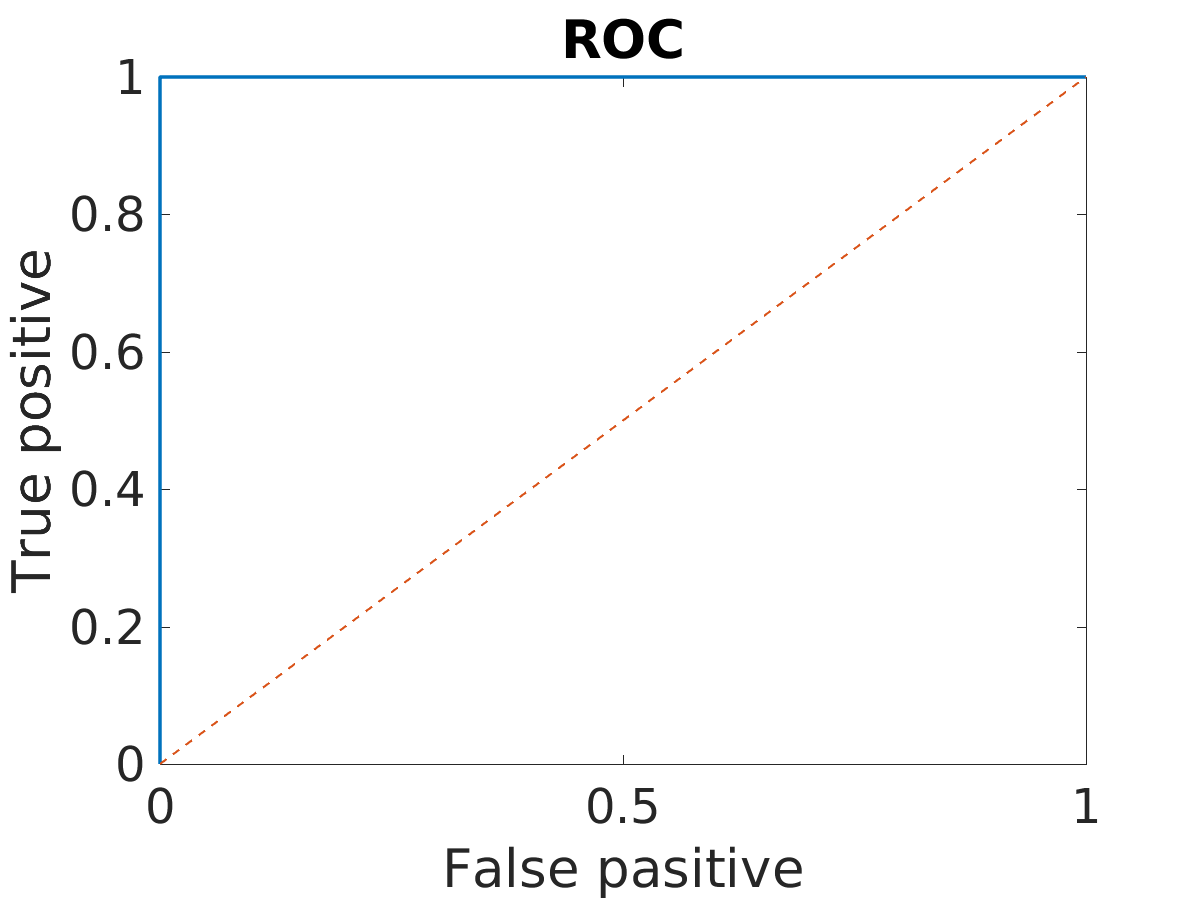
\includegraphics[width=0.6\textwidth]{./img/ROC/ROC_gauss_synt_3_50.png}
\caption{\small{ROC curve of a synthetic view created at distance equal to baseline/2 marked with power equal to 3 }}
\label{fig:g3vs50}
\end{figure}
\begin{figure}[h!]
\centering
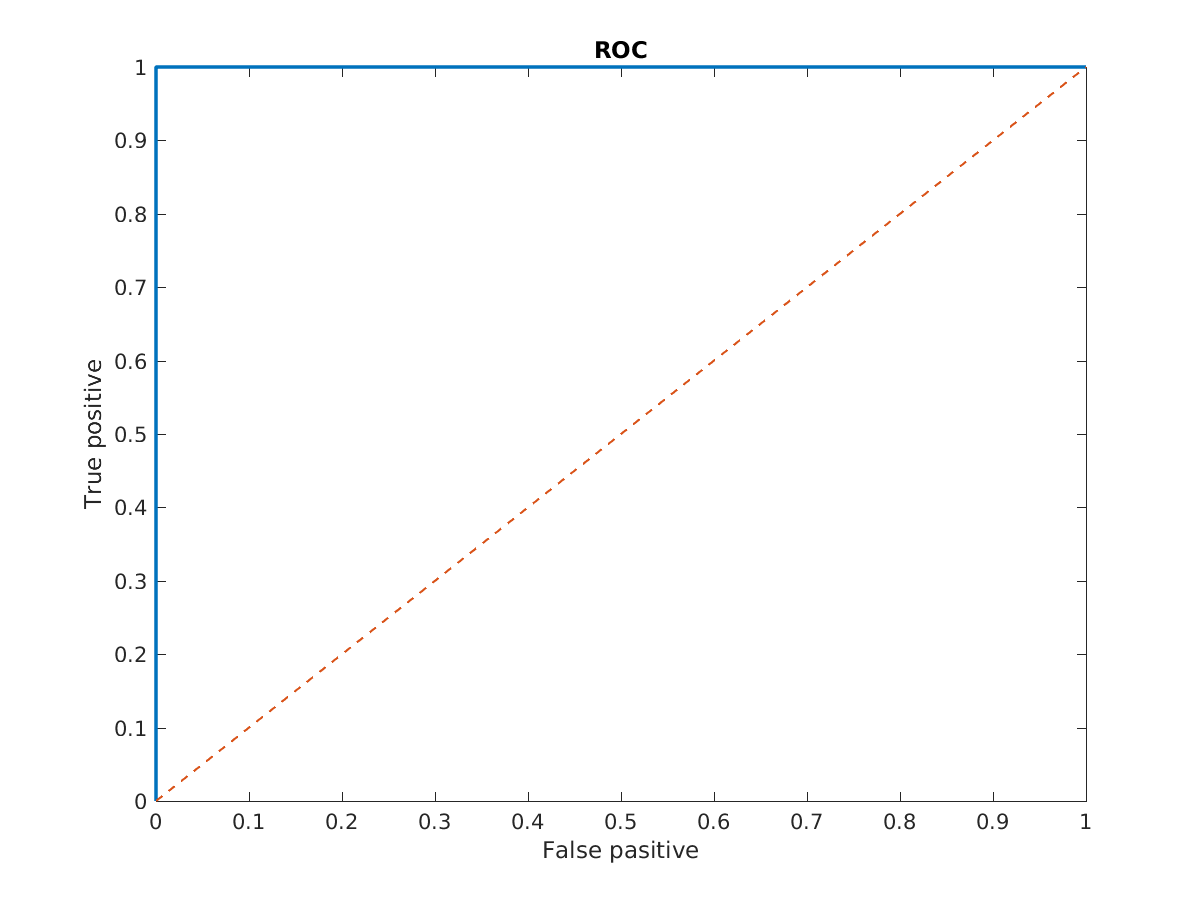
\includegraphics[width=0.6\textwidth]{./img/ROC/ROC_gauss_synt_3_75.png}
\caption{\small{ROC curve of a synthetic view created at distance equal to baseline*3/4 marked with power equal to 3 }}
\label{fig:g3vs75}
\end{figure}
\clearpage
It can be noted that the detection statistics are very high in the synthetized views, either for the spatial and frequency technique; we can therefore expect the synthetized views to behave like the other against compression.\newline

Often with stereo watermarking, view synthesis can be a problem since it introduces non-rigid local geometric distortion that are not properly tackled by state-of-the art resynchronization mechanisms. Local geometric deformations destroys the synchronization necessary for the detection process to be succesful.

With the proposed method the detection of the watermark in the right view works by warping it according to the disparity; this way the resynchronization is an internal step of the detection process and it doesn't need side information to resynchronize the watermark, since the disparity can be estimated anytime from the received views.
\newline Therefore we can say that this strategy manages to achieve complete robustness to view synthesis.
\clearpage
\section{Perceptual impact}

As said in Chapter \ref{wat} the perceptual impact, i.e. the imperceptivity of the watermark to the human eye, has been measure with the metrics proposed by Chaminda et al \cite{QMETRICS}.\\ 
This test is motivated by the fact that researchers have found out that there is a strong correlation between subjective 3D video quality ratings and candidate objective quality measures (e.g., video quality metric (VQM), peak-signal-to-noise ratio (PSNR), structure similarity metric (SSIM)) of individual image components of 3D video, e.g., PSNR values of color image and corresponding depth map or average PSNR of left and right view images. This means that we can use individual objective quality ratings of 3D video components in place of time consuming subjective test procedures for most of the system parameter changes with a reasonable accuracy.\\
In particular the study in \cite{QMETRICS} is based on the fact that the edges/contours of the depth map can be considered for measuring structural degradation, it is proposed a metric which is a modified version of the SSIM metric. In  \cite{QMETRICS} this measure is computed on the degradated view and the corresponding disparity map, in our case we measured either the degradataion on the left and right view.

Figure \ref{fig:sobel} gives graphical illustration of contour extraction in order to compute the RR metrics on the left view, in this case the image has been marked with power equal to 0.3 and it can be noted that this kind of watermarking doesn't affect the contours of the scene.
   
\begin{figure}[h!]
\centering
\begin{subfigure}[]{0.4\textwidth}
\centering
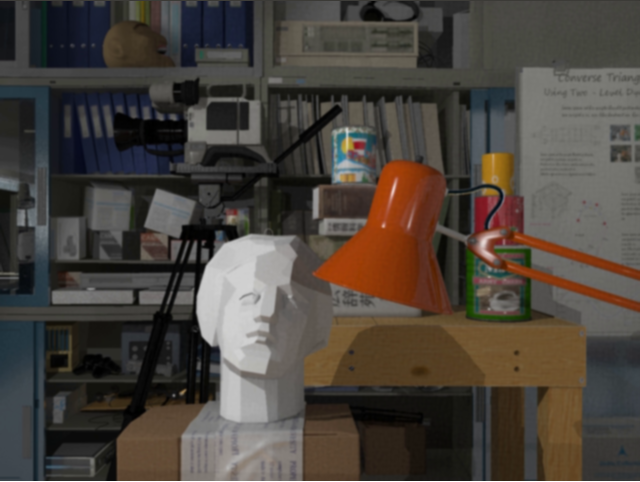
\includegraphics[width=0.9\textwidth]{./img/wat_left.png}
\caption{\label{fig:lw}}
\end{subfigure}
\begin{subfigure}[]{0.4\textwidth}
\centering
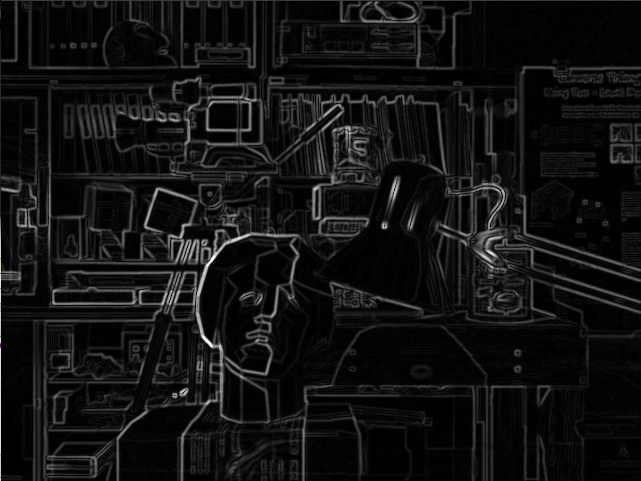
\includegraphics[width=0.9\textwidth]{./img/left_sobel.png}
\caption{\label{fig:lws}}
\end{subfigure}
\begin{subfigure}[]{0.4\textwidth}
\centering
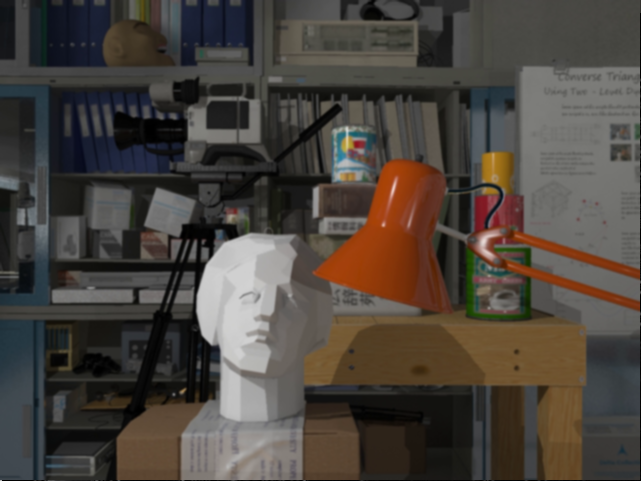
\includegraphics[width=0.9\textwidth]{./img/right_wat.png}
\caption{\label{fig:wr}}
\end{subfigure}
\begin{subfigure}[]{0.4\textwidth}
\centering
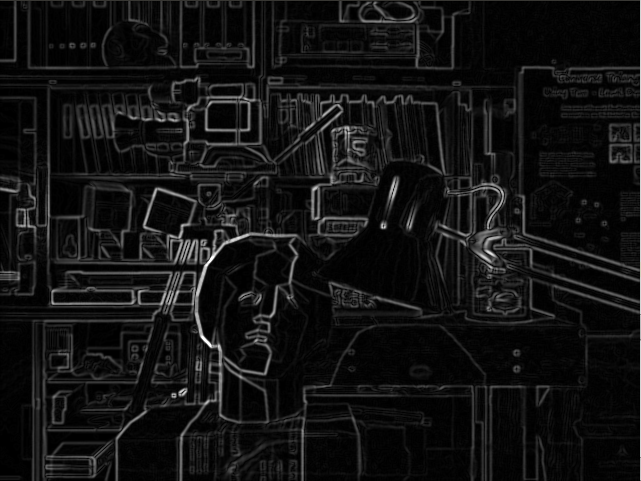
\includegraphics[width=0.9\textwidth]{./img/right_sobel.png}
\caption{\label{fig:rws}}
\end{subfigure}
\begin{subfigure}[]{0.4\textwidth}
\centering
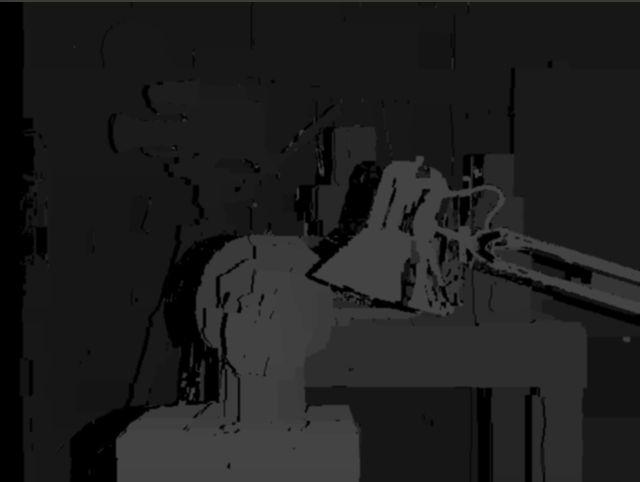
\includegraphics[width=0.9\textwidth]{./img/ldisp.png}
\caption{\label{fig:ld}}
\end{subfigure}
\begin{subfigure}[]{0.4\textwidth}
\centering
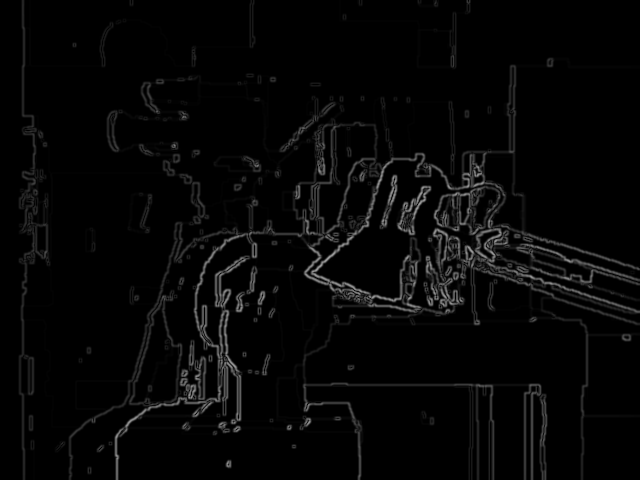
\includegraphics[width=0.9\textwidth]{./img/ldisp_sobel.png}
\caption{\label{fig:lds}}
\end{subfigure}
\begin{subfigure}[]{0.4\textwidth}
\centering
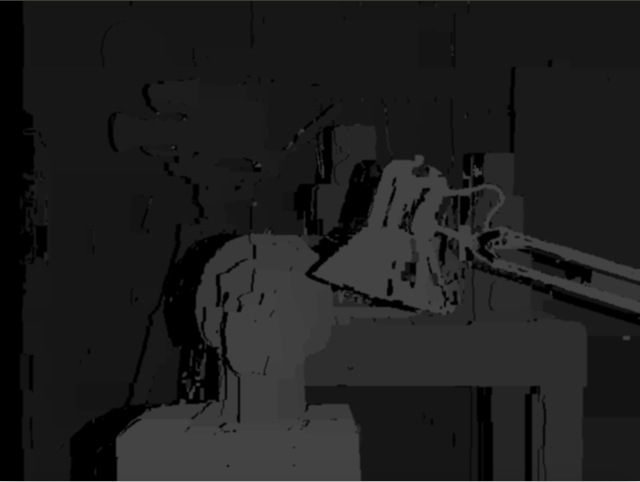
\includegraphics[width=0.9\textwidth]{./img/rdisp.png}
\caption{\label{fig:rd}}
\end{subfigure}
\begin{subfigure}[]{0.4\textwidth}
\centering
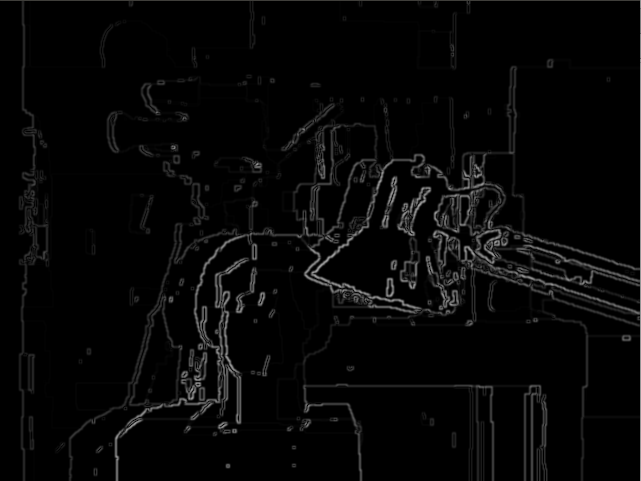
\includegraphics[width=0.9\textwidth]{./img/rdisp_sobel.png}
\caption{\label{rds}}
\end{subfigure}
\caption{\small{(a) Reference left image. (b) Extracted edge information from reference left image. (c) Watermarked left image. (d) Extracted edge information from the watermarked left image. (e) Left disparity map obtain from the non watermarked stereo pair. (f) Extracted edge information from the left disparity map obtain from the non watermarked stereo pair. (g)  Left disparity map obtain from the watermarked stereo pair.(h) Extracted edge information from the left disparity map obtain from the watermarked stereo pair. }\label{fig:sobel}}
\end{figure}
\clearpage
For different power of watermarking both the $MQ_{depth}$ and $MQ_{color}$ metrics are calculated, and in figures \ref{fig:qml}-\ref{fig:qmr} its shown the value of the quality measure with respect to the increasing value of the watermark power. 

\begin{figure*}[h!]
    \centering
    \begin{subfigure}[t]{0.5\textwidth}
        \centering
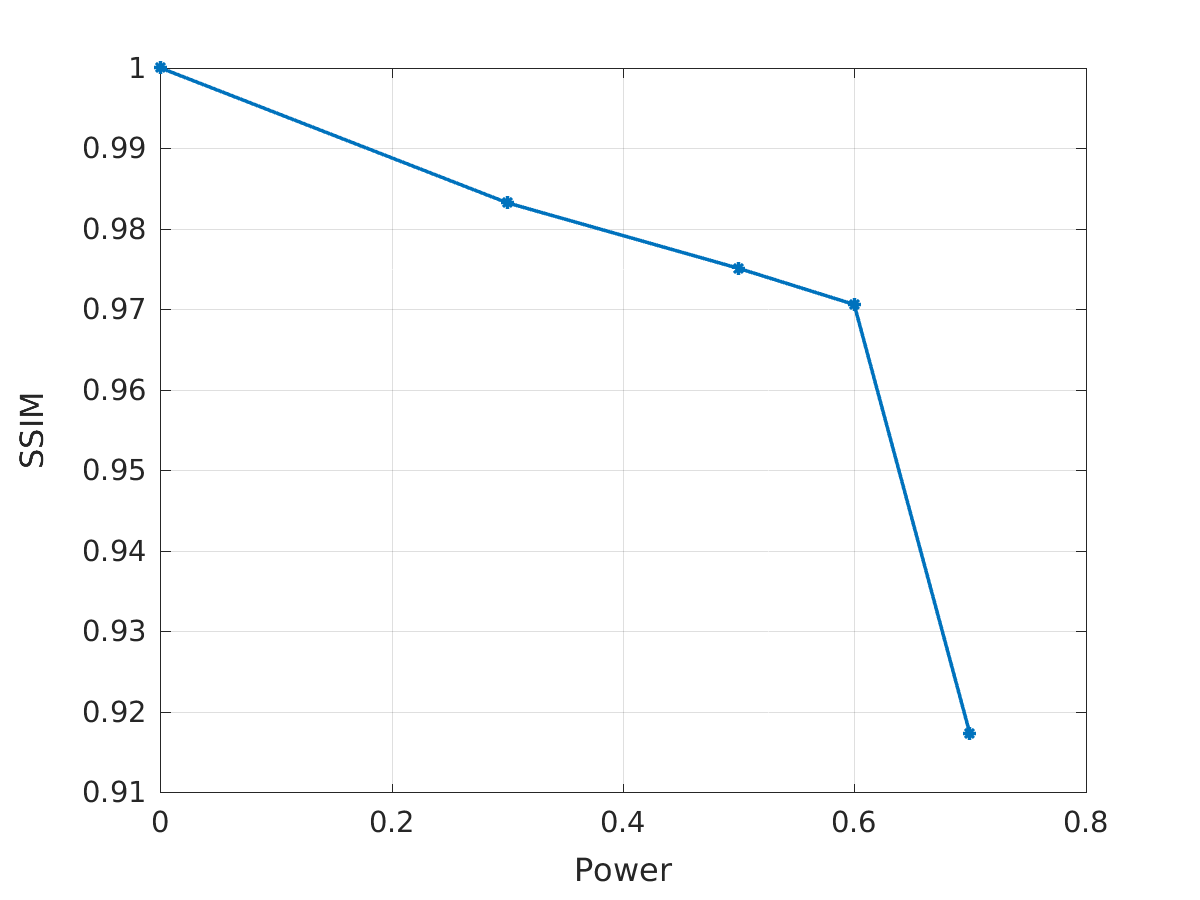
\includegraphics[width=1\textwidth]{./img/qm/qm_left.png}
          \caption{\small{Color quality metrics on the left view}}
\label{fig:qmcl}

    \end{subfigure}%
    ~ 
    \begin{subfigure}[t]{0.5\textwidth}
        \centering
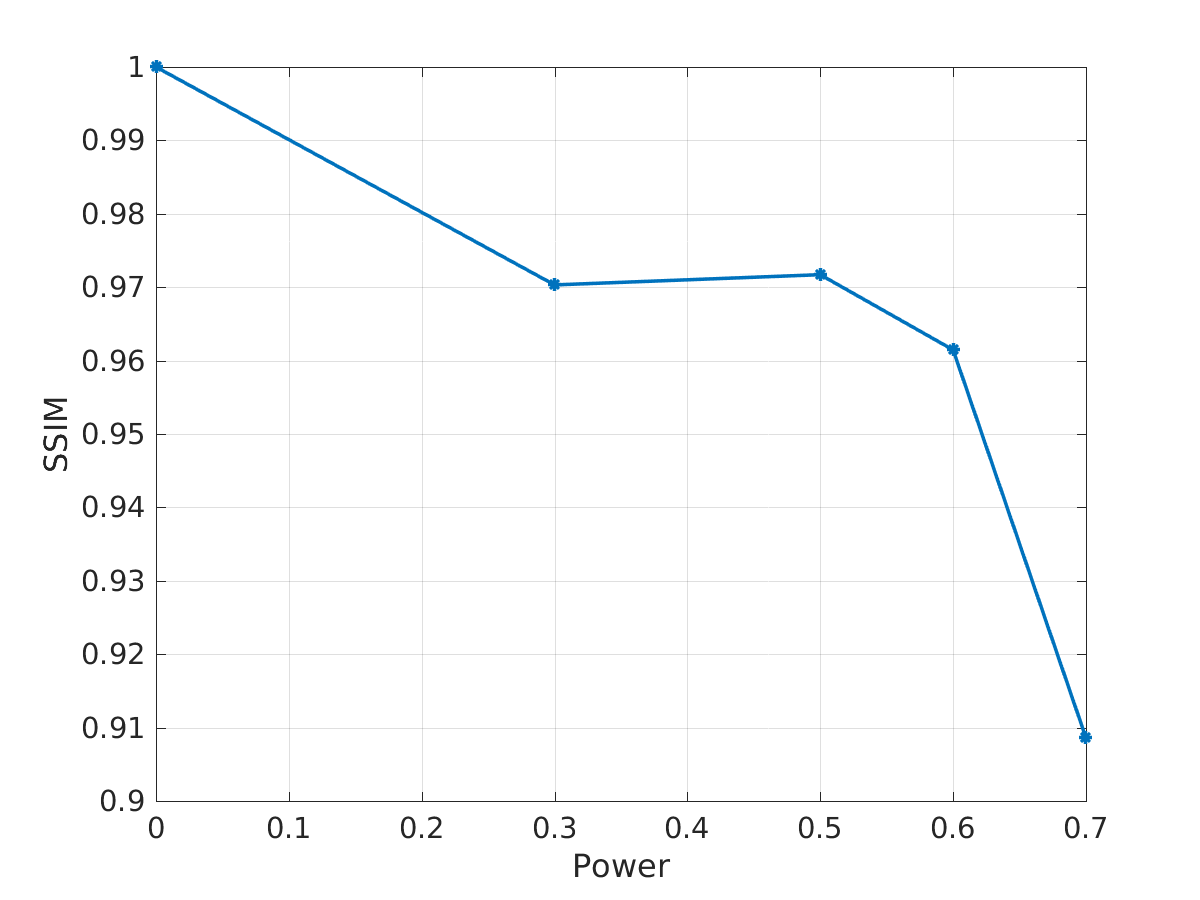
\includegraphics[width=1\textwidth]{./img/qm/qm_disp_left.png}
           \caption{\small{Color quality metrics on the right view}}
\label{fig:qmdl}
    \end{subfigure}
    \caption{Color Quality metrics}
    \label{fig:qml}
\end{figure*}

\begin{figure*}[h!]
    \centering
    \begin{subfigure}[t]{0.5\textwidth}
        \centering
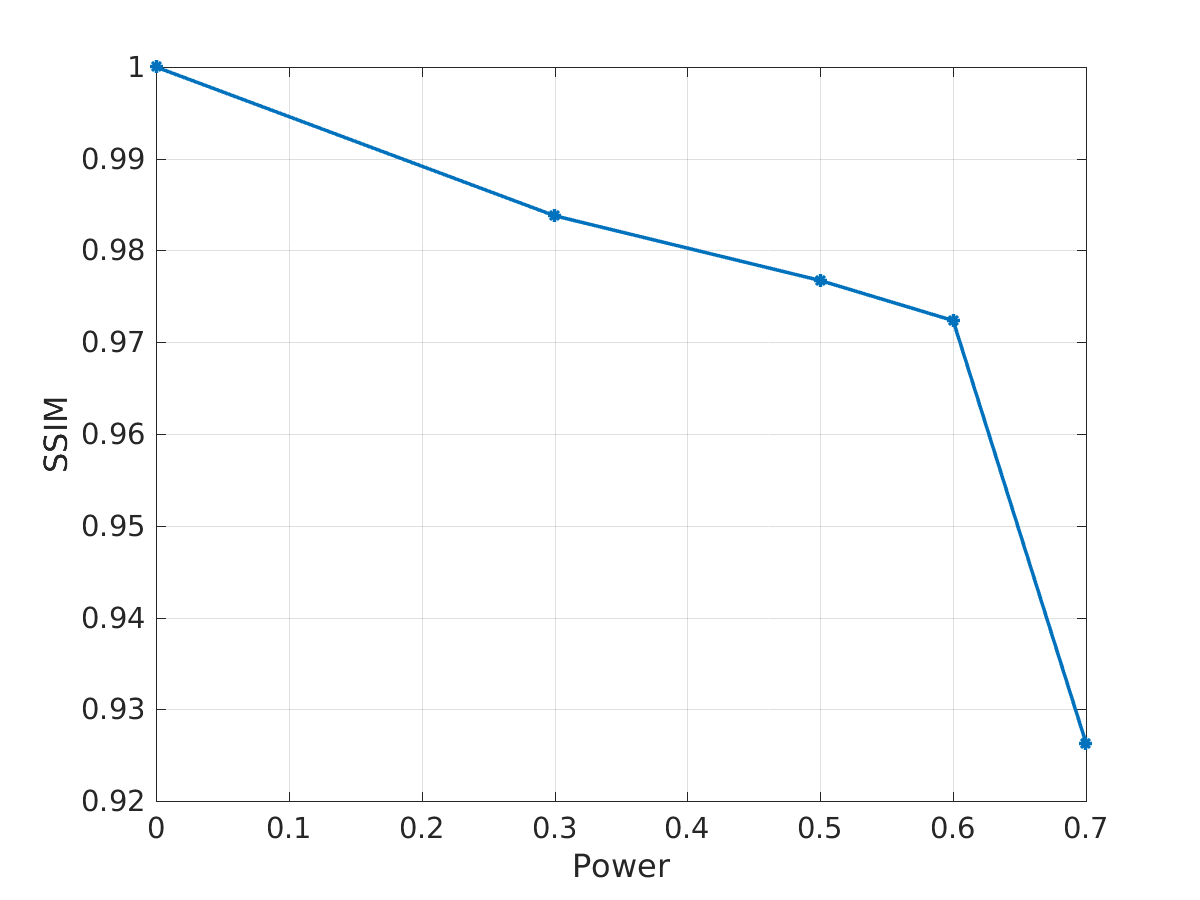
\includegraphics[width=1\textwidth]{./img/qm/qm_right.png}
          \caption{\small{Depth quality metrics on the left view}}
\label{fig:qmcr}

    \end{subfigure}%
    ~ 
    \begin{subfigure}[t]{0.5\textwidth}
        \centering
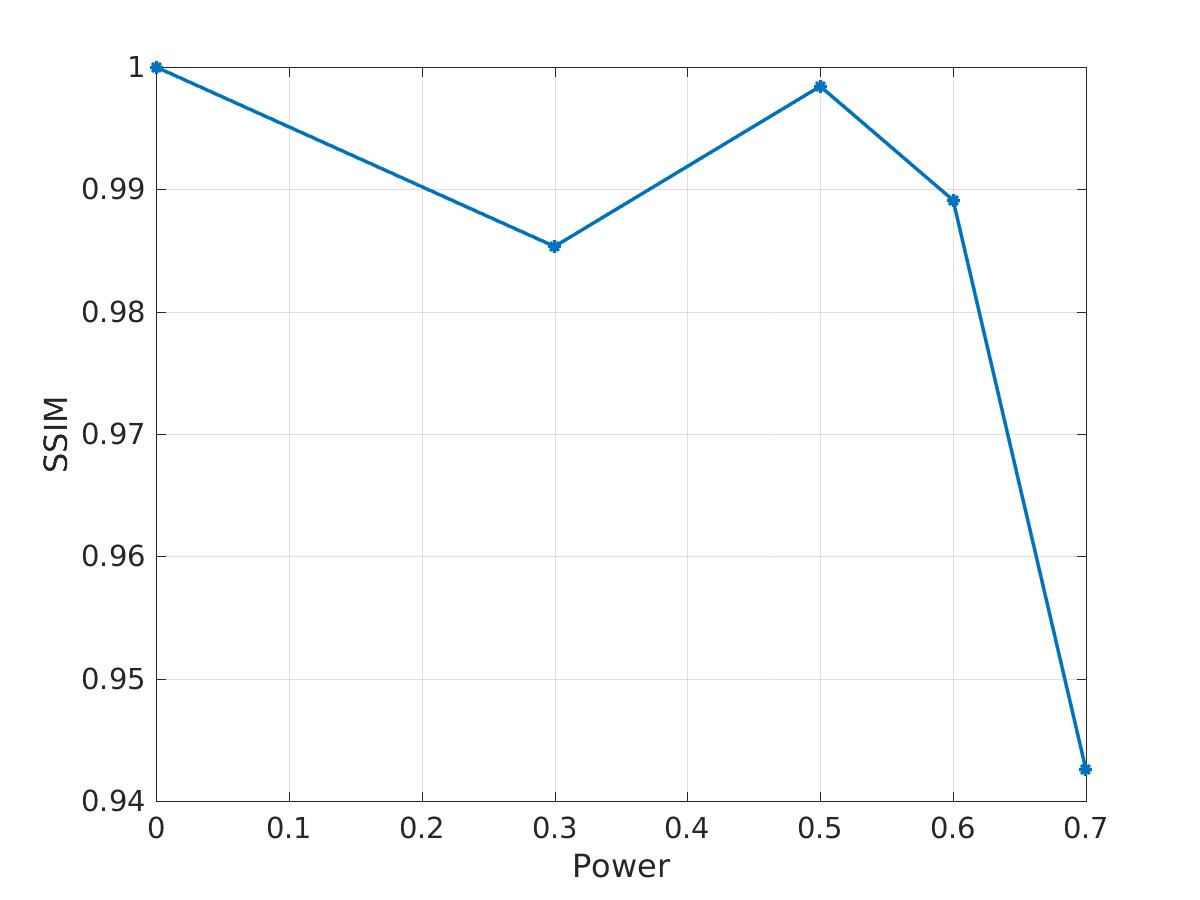
\includegraphics[width=1\textwidth]{./img/qm/qm_disp_right.png}
           \caption{\small{Depth quality metrics on the right view}}
\label{fig:qmdr}
    \end{subfigure}
    \caption{Depth quality metrics }
        \label{fig:qmr}
\end{figure*}
\clearpage

In figures \ref{fig:qml}-\ref{fig:qmr} we can see how the quality metrics decrease when increasing the power of the watermark: it can be noted that the more the power of the watermark is high the more the quality of the perception is low, however with power lower the 0.6 the degradation mantain an acceptable level with respect to the value generated from the non marked image (power equal to 0).

\subsection{PSNR test}

Another study has been conducted to evaluate the visual impact of the watermark: the average PSNR value has been computed between the I frames of the original stereoscopic video and the watermarked stereoscopic videos with different values of the power(that is 30 pairs of stereoscopic frames).\\
As said before typical values for the PSNR in video watermarking are between 30 and 50 dB.
The results of this study are shown in Table \ref{tab:psnr_wm}: with a power value of $0.3$ PSNR reaches a maximum value of $44.438$, which indicates a good quality of the watermarked stereo pair. \\
As expected the PSNR value decrease with the increment of the watermaking power, indicating a degratation of the watermarked videos.\\ This analysis is in line with the one conducted with the quality metrics in \cite{QMETRICS}.

\begin{table}[h!]
\begin{center}
\scalebox{0.9}{ 
\begin{tabularx}{0.7\textwidth}{>{\centering\arraybackslash}X>{\centering\arraybackslash}X}
\hline \hline
Power & PSNR(dB) \\ \hline
0.3 & 46.0071 \\  					
0.5 & 45.9505 \\
0.6& 45.9291 \\
\hline 
\end{tabularx}
 }
\caption{\small{Average PSNR values between original video and watermarked videos with increasing value of the power.} \label{tab:psnr_wm}}
\end{center}
\end{table}
\clearpage
\section{Remarks}

In this chapter the experiments conducted to test the proposed watermarking technique have been presented.

First we proved the uniqueness of the watermark needed in order to have a reliable marking process.

The created stereo video sequence was than watermarked and compressed under different compression rates, to test the visibility of the watermark as well as its robustness against lossy compression.

Regarding the spatial technique, results show that when the watermark is added with power equal to 1, it is preserved with acceptable statistic at a compression rate of 15; on the other hand when inserted with higher power (3 in this analysis), the detection statistics are optimal even for the crudest compression of crf 30. 

The frequency watermarking proved to be robust up to a compression rate of 25, and that the degradation introduced by web uploading tends to erase the mark, so in order to cope with this kind of attack a higher embedding power is needed.

The quality of the watermarked video has been studied with Reduced Reference quality metrics \cite{QMETRICS}, based on the $MQcolor$ graph we can make the following observations: in the frequency domain, if we fix a loss of quality of $1\%$ with respect to the non marked video, we obtain an embedding power of $0.3$, in Table \ref{tab:03} are shown the detection statistic in this case. If we accept a degradation of $3\%$ we obtain an acceptable embedding power of $0.6$, this statistics are shown in Table  \ref{tab:06}. 

From the study conducted for the spatial domain it emerges that an acceptable degratation can only be obtained with embedding strenght equal to 1, in this case we study the distribution of True Positive detection with respect to increasing compression powwer; results are shown in Table \ref{tab:G1}.


\begin{table}[htbp]
 
 \begin{center}
 \scalebox{0.9}{ 
 \begin{tabular}{c|c c c }
 \hline\hline
 \multirow{1}{2.5cm}{\textbf{$CRF$}} &  \multirow{1}{2.5cm}{\textbf{$power$}} & \multicolumn{1}{c}{\textbf{$PD_{True Positive}$}} \\ \hline

1& 1 &  \\
15& 1 & \\
25& 1 & \\
30& 1 & \\
 \hline
 \end{tabular}
 }
 \caption{\label{tab:G1}}
 \end{center}
 \end{table}


\begin{table}[htbp]
 
 \begin{center}
 \scalebox{0.9}{ 
 \begin{tabular}{c|c c c }
 \hline\hline
 \multirow{1}{2.5cm}{\textbf{$CRF$}} &  \multirow{1}{2.5cm}{\textbf{$power$}} & \multicolumn{1}{c}{\textbf{$Detected frames$}} \\ \hline

1& 0.3 & 30  \\
15& 0.3 & 29 \\
25& 0.3 & 11 \\
30& 0.3 & 2\\
 \hline
 \end{tabular}
 }
 \caption{\label{tab:03}}
 \end{center}
 \end{table}
 
 \begin{table}[htbp]
 \begin{center}
 \scalebox{0.9}{ 
 \begin{tabular}{c|c c c }
 \hline\hline
 \multirow{1}{2.5cm}{\textbf{$CRF$}} &  \multirow{1}{2.5cm}{\textbf{$power$}} & \multicolumn{1}{c}{\textbf{$Detected frames$}} \\ \hline

1& 0.6 &  30\\
15& 0.6 & 30 \\
25& 0.6 & 26\\
30& 0.6 & 15\\
 \hline
 \end{tabular}
 }
 \caption{\label{tab:06}}
 \end{center}
 \end{table}

Another important feature to test was the robustness against view synthesis, which was confirm by the results, for both the spatial and frequency techniques.



Finally the average PSNR value has been computed to analyse compression and visual impact of the watermark; the study supports the previous results. 


